% updated April 2002 by Antje Endemann
% Based on CVPR 07 and LNCS, with modifications by DAF, AZ and elle, 2008 and AA, 2010, and CC, 2011; TT, 2014; AAS, 2016; AAS, 2020; TH, 2022
%\pdfoutput=1\relax%XeLaTeX-compat: use \ifpdf\pdfoutput1\fi
\documentclass[runningheads]{llncs}
\usepackage[dvipsnames,table]{xcolor}
\usepackage{graphicx}
% DO NOT USE \usepackage{times}, it will be removed by typesetters
%\usepackage{times}

\usepackage{tikz}
\usepackage{comment}
\usepackage{amsmath,amssymb} % define this before the line numbering.
\usepackage{color}
\usepackage[pagebackref,breaklinks,colorlinks]{hyperref}
\hypersetup{citecolor=[RGB]{119,185,0}}
\usepackage{tabularx,booktabs}
\usepackage{multirow}
\usepackage{pifont}
\usepackage{subfigure}
% \usepackage{subcaption}
\usepackage{breakcites}

% \sloppy

% The "axessiblity" package can be found at: https://ctan.org/pkg/axessibility?lang=en
%\usepackage[accsupp]{axessibility}  % Commented out for XeLaTeX compatibility

% INITIAL SUBMISSION - The following two lines are NOT commented
% CAMERA READY - Comment OUT the following two lines
% \usepackage{ruler}
% \usepackage[width=122mm,left=12mm,paperwidth=146mm,height=193mm,top=12mm,paperheight=217mm]{geometry}

\newcommand{\cl}[1]{\textcolor{magenta}{[CL]: #1}}
\newcommand{\hsc}[1]{\textcolor{red}{[#1]}}



% Chinese support (auto-injected)
\usepackage{xeCJK}
\setCJKmainfont{Noto Serif CJK SC}[ItalicFont=AR PL UKai TW MBE]
\setCJKsansfont{Noto Sans CJK SC}
\setCJKmonofont{Noto Sans CJK SC}
\raggedbottom
\renewcommand{\figurename}{图}
\renewcommand{\tablename}{表}
\renewcommand{\abstractname}{摘要}
\renewcommand{\refname}{参考文献}
\begin{document}
% \renewcommand\thelinenumber{\color[rgb]{0.2,0.5,0.8}\normalfont\sffamily\scriptsize\arabic{linenumber}\color[rgb]{0,0,0}}
% \renewcommand\makeLineNumber {\hss\thelinenumber\ \hspace{6mm} \rlap{\hskip\textwidth\ \hspace{6.5mm}\thelinenumber}}
% \linenumbers
\pagestyle{headings}
\mainmatter
\def\ECCVSubNumber{1807}  % Insert your submission number here

%\title{Triple-boosting Autonomous Driving in \\ 
%an End-to-end Vision-based Framework } % Replace with your title
%\title{ST-P3: End-to-end Vision-based Autonomous Driving via Spatial-temporal Co-optimization} % Replace with your title
\title{ST-P3：基于时空特征学习的端到端视觉自动驾驶} % Replace with your title
% INITIAL SUBMISSION 
\begin{comment}
\titlerunning{ECCV-22 submission ID \ECCVSubNumber} 
\authorrunning{ECCV-22 submission ID \ECCVSubNumber} 
\author{Anonymous ECCV submission}
\institute{Paper ID \ECCVSubNumber}
\end{comment}
%******************

% CAMERA READY SUBMISSION
% \begin{comment}
\titlerunning{ST-P3}
% If the paper title is too long for the running head, you can set
% an abbreviated paper title here
%
\author{Shengchao Hu\inst{1}$^\dagger$ \and
Li Chen\inst{2}$^\ast$ \and
Penghao Wu\inst{1,3}$^\dagger$ \and
Hongyang Li\inst{1,2} \and \\
Junchi Yan\inst{1,2} \and
Dacheng Tao\inst{4}
}
% \author{First Author\inst{1}\orcidID{0000-1111-2222-3333} \and
% Second Author\inst{2,3}\orcidID{1111-2222-3333-4444} \and
% Third Author\inst{3}\orcidID{2222--3333-4444-5555}}
%
\authorrunning{S. Hu et al.}
% First names are abbreviated in the running head.
% If there are more than two authors, 'et al.' is used.
%
\institute{教育部人工智能重点实验室，上海交通大学 \and
上海人工智能实验室，上海，中国 \and
加州大学圣地亚哥分校，加利福尼亚，美国 \and
京东探索研究院，京东集团股份有限公司，北京，中国 \\
\email{charles-hu@sjtu.edu.cn}\quad 
\email{lichen@pjlab.org.cn}
}
% \institute{Princeton University, Princeton NJ 08544, USA \and
% Springer Heidelberg, Tiergartenstr. 17, 69121 Heidelberg, Germany
% \email{lncs@springer.com}\\
% \url{http://www.springer.com/gp/computer-science/lncs} \and
% ABC Institute, Rupert-Karls-University Heidelberg, Heidelberg, Germany\\
% \email{\{abc,lncs\}@uni-heidelberg.de}}
% \end{comment}
%******************
\maketitle

\let\thefootnote\relax\footnote{$^\ast$ 通讯作者。$^\dagger$ 工作完成于上海人工智能实验室实习期间。}

\begin{abstract}
现有自动驾驶范式大多采用多阶段离散任务流水线。为更好预测控制信号并提升用户安全性，一种能从联合时空特征学习中受益的端到端（End-to-end）方法十分必要。尽管已有一些基于 LiDAR（LiDAR）输入或隐式设计的先驱工作，本文在一个可解释的视觉设置下对问题进行建模。具体而言，提出一种时空（Spatial-temporal）特征学习方案，为感知（Perception）、预测（Prediction）和规划（Planning）任务同时学习更具代表性的特征，称为 ST-P3（ST-P3）。其中，提出一种自我中心对齐累积（Egocentric Aligned Accumulation）技术，在鸟瞰图（Bird's eye view, BEV）变换前保留 3D 空间几何信息；设计一种双路径建模（Dual Pathway Modelling）方法，将过去运动变化纳入未来预测；引入一个基于时序的优化单元，补偿规划中对视觉元素的识别。据本文所知，首次系统性地研究了可解释端到端视觉自动驾驶系统的各个部分。在开环（Open-loop）nuScenes（nuScenes）数据集和闭环（Closed-loop）CARLA（CARLA）仿真上对方法进行了基准测试，与最先进方法（State-of-the-art, SOTA）对比。结果表明了本文方法的有效性。源代码、模型和协议细节已在 \url{https://github.com/OpenPerceptionX/ST-P3} 公开。

% \keywords{End-to-end autonomous driving, Bird's eye view perception, Motion prediction, Learning-based planning}
\end{abstract}


\section{引言}\label{sec: intro}




经典自动驾驶系统设计通常采用模块化流水线范式\cite{behere2015functional,yurtsever2020survey}，其中规划或控制单元输入依赖于上游感知（Perception）模块输出。
%
随着端到端（End-to-end）算法蓬勃发展并在多个领域成功应用\cite{pfeiffer2017perception,hamalainen2019affordance}，自动驾驶领域也出现了类似尝试\cite{pomerleau1988alvinn,bojarski2016end,openpilot,bansal2018chauffeurnet,chitta2021neat,prakash2021multi,zhang2021end,chen2021wor,chen2022lav}。
%
本文目标并非孤立的分阶段流水线，而是一个直接以原始传感器数据为输入、生成规划路径或控制信号的框架。
%
这样做的一个直观动机是：特征表示可在	extit{同一}网络内被联合优化，以服务于系统最终目标（如加速、转向）。
%

端到端流水线的一个方向是主要聚焦于最终规划任务，而不对中间表示进行显式设计\cite{codevilla2018end,codevilla2019exploring,prakash2021multi,chen2020learning,chitta2021neat,hu2021safe}。
%
强化学习（RL）作为一种可行方案十分契合，因为规划路径不唯一，各动作应根据环境获得相应奖励。
%
RL算法被用于模仿经验丰富的人类专家，引导驾驶智能体（Agent）行为学习\cite{zhang2021end,Chekroun2021gri}。
除RL方法外，也有工作提出利用感知环境知识生成代价图（Cost map）与轨迹采样器（Trajectory sampler）\cite{hu2021safe,chitta2021neat}，或以注意力机制融合多传感器信息\cite{prakash2021multi,fadadu2022multi}。
%
上述工作在闭环仿真中取得了令人瞩目的性能\cite{dosovitskiy2017carla}，但从合成环境到真实应用的可迁移性仍是开放问题。

另一方向是在网络中显式设计中间表示，为各模块提供令人信服的可解释性，从而增强系统稳定性和安全性。基于输入类型，显式方法可分为基于 LiDAR（LiDAR）的\cite{casas2021mp3,zeng2020dsdnet,zeng2019end,cui2021lookout}和基于视觉的\cite{hu2021fiery,philion2020lift,wang2021learning}。
%
结合高清地图（High-definition map, HD map）的 LiDAR 方法在多种基准上表现良好，并系统性地研究了系统各模块效果。但 LiDAR 的固有限制——如对交通信号灯的识别和近距离物体检测——可能限制其应用。
%

本文与具备可解释性的 LiDAR 流水线\cite{casas2021mp3,zeng2020dsdnet}并行，提出探索	extit{基于视觉}的端到端框架（图 \ref{fig:motivation}）的潜力。
%
若各模块经过精细设计，感知、预测和规划各任务的性能可提升到何种程度？



\begin{figure}[tb!]
    \centering
    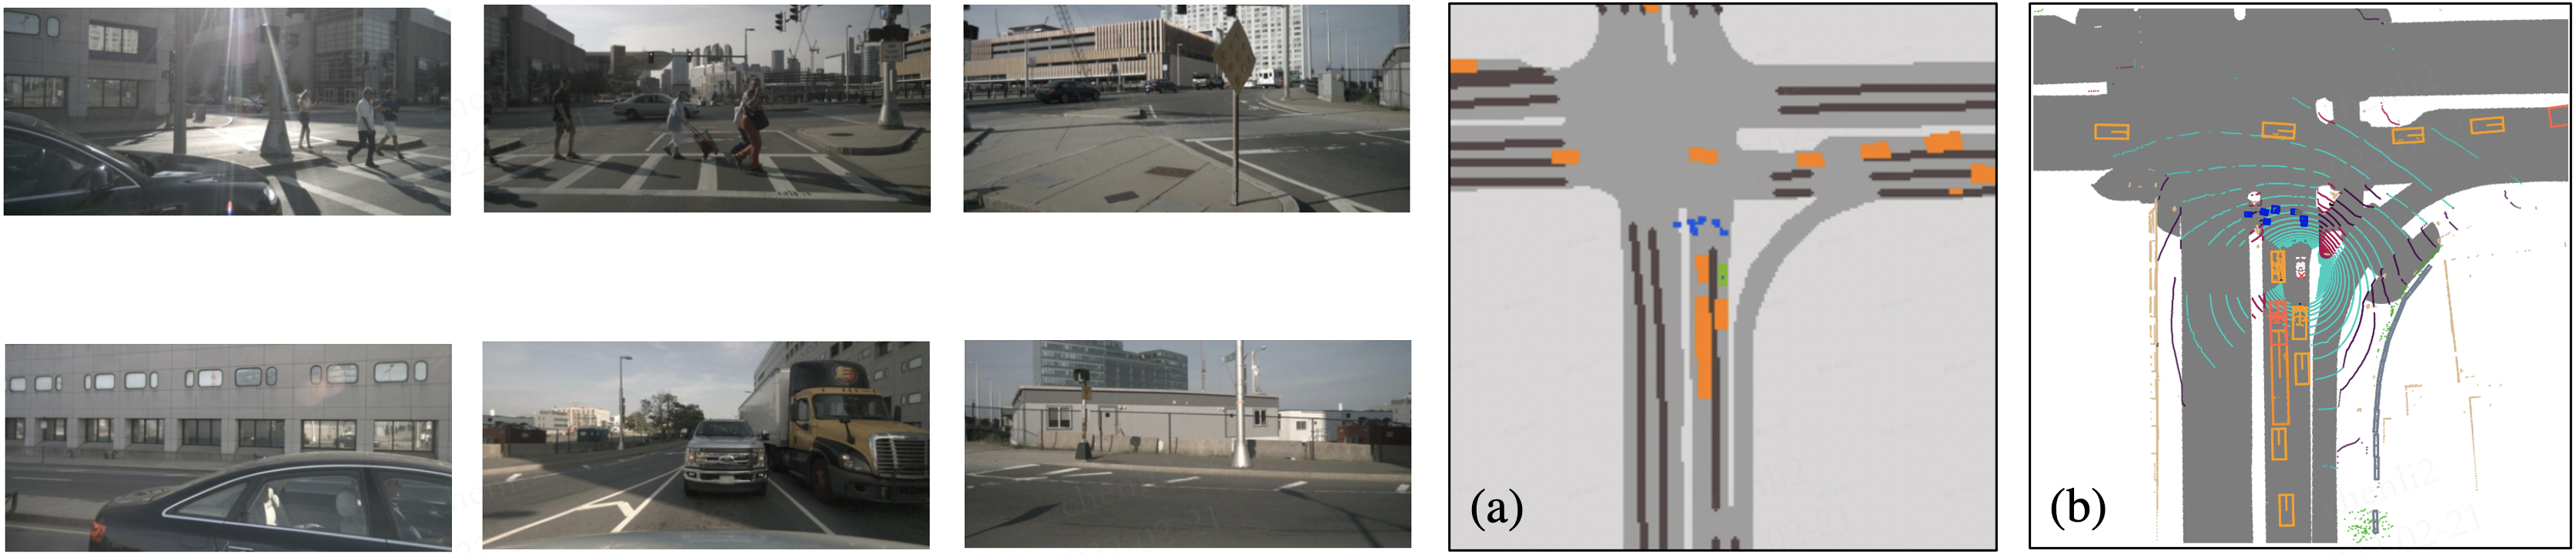
\includegraphics[width=1.\textwidth]{Figs/motivation.png}
    % \vspace{-.7cm}
    \caption{问题设定：图 (a) 中设计的可解释视觉端到端框架，与图 (b) 中借助高清地图（HD map）的 LiDAR 方法并行
    }
    \label{fig:motivation}
    % \vspace{-.4cm}
\end{figure}

% Implicit methods~\cite{codevilla2018end,codevilla2019exploring,prakash2021multi} directly map the input sensor data to planned trajectory or control signal \textit{without} utilizing any explicit intermediate representations. 
% %
% However, they suffer from the lack of interpretability, making it hard to guarantee security.

% Given the target point, the autonomous system should produce a safe and comfortable trajectory getting to the determination. 
% With the successful application in computer vision tasks, deep learning technology has also been applied to the self-driving which takes the raw sensor input (e.g., LiDAR, image) to output the control command,\textit{ e.g.}, acceleration, brake and steering.  However, most autonomous companies treat this problem as several subtasks: perception, prediction, planning and control, and then each module is dedicated by one team in isolation. 
% This may cause  accumulation loss and the promotion of one sub-tasks does not mean the promotion of all the system. In the meantime, end-to-end approach has shown its potentiality and efficiency though it has not yet been in massive production, due to the joint optimization of all modules and focus on the final objective: planning and control. The success of the Openpilot~\cite{openpilot} also shows its effectiveness.

% The early attempts in end-to-end approach directly map the sensor input to the control command~\cite{bojarski2016end,pomerleau1988alvinn} or planning trajectory~\cite{bansal2018chauffeurnet,chen2020learning}. In order to improve the interpretability and the ability to handle complex situation, some researchers incorporate some auxiliary tasks into their methods. For example, NEAT~\cite{chitta2021neat} outputs the waypoint and semantics at the same time to improve the interpretability of its attention maps,  and therefore obtains competitive driving scores in the CARLA simulator~\cite{dosovitskiy2017carla}. Meantime, Transfuser~\cite{prakash2021multi} explores the sensor fusion methods to get more surrounding information and uses the attention to integrate image and LiDAR representations, and validates its efficacy in the CARLA urban driving simulator. However, these methods though include the auxiliary tasks or do the sensor fusion, they still lack of the interpretability of how the trajectory generated.

% In order to give convincing trajectory, the NMP~\cite{zeng2019end} first attempts to use the cost map to score the trajectory and thus we can explicitly see the process of the trajectory generation. However, the cost map is learned by the neural network which is still lack of interpretability.  P3~\cite{sadat2020perceive} exploits a novel semantic layer as intermediate interpretable representation which can be used to penalize unsafe maneuvers. And MP3~\cite{casas2021mp3} further expands application scenarios by discarding the High-definition maps (HD maps) information.  However MP3 is LiDAR-based method and do not include the camera information which is important for the traffic light detection. In addition, due to the LiDAR inherent defect, MP3  can not detect the long distance objects which may cause untimely reaction to some situation, e.g. the collision in the highway which need brake in advance. Some may resort to the sensors fusion to incorporate all sensors data into the network~\cite{fadadu2022multi,liang2019multi,liang2018deep,zhou2020end}, while it is hard to align all sensors in space and time, and the performance of sensor fusion is still lack of proof.

% To address these challenges, we propose an end-to-end multi-view camera-based approach to mapless driving which only inputs the camera and produces a safe and comfortable trajectory. The intermediate representations are all interpretable and reserved for the trajectory planning. IVMP~\cite{wang2021learning} follows the same setting and obtains competitive results on the nuScenes dataset~\cite{caesar2020nuscenes} and CARLA simulator. Intuitively, the accuracy of the intermediate results affect the safety of the planning, for example, the higher the accuracy of predicting the vehicle's segmentation, the safer the planned trajectory. In this paper we take a different approach to obtain better results in most intermediate representations and finally obtain safer trajectory.


为回答上述问题，基于视觉的方法首要挑战是如何将特征表示从透视图（Perspective view）变换到鸟瞰图（Bird's eye view, BEV）空间。
%
先驱工作 LSS\cite{philion2020lift} 从多视角相机提取透视图特征，通过深度估计（Depth estimation）将其提升至 3D 空间并融合到 BEV 空间。研究表明，两视图间的特征变换中隐式深度预测至关重要\cite{hu2021fiery,wang2021learning,reading2021CaDDN}。从理论分析看，这具有合理性——将 2D 平面信息提升到 3D 需要额外维度，即符合 3D 几何自动驾驶任务的深度。
%
为进一步提升特征表示，很自然地应将时序信息纳入框架，因为大多数场景涉及视频源。
继 LSS\cite{philion2020lift} 之后，后续工作通过自动驾驶车辆（Self-driving vehicle, SDV）的自车运动（Ego-motion）（由数据集提供）\cite{hu2021fiery}或光流学习映射\cite{wang2021learning}，将过去帧特征投影到当前坐标视图。
%
这些方法将过去帧特征逐帧独立投影，然后馈入时序模型（Temporal model）；而本文在变换到 BEV 前将所有过去对齐特征累积在 3D 空间，最大程度保留几何信息并补偿当前状态特征表示的鲁棒性。实验证实这是更优的设计选择，尤其对静态物体。



% %
% FIERY~\cite{hu2021fiery} builds upon LSS and further incorporates features in the past frames to the present by a Spatial Transformer Network~\cite{jaderberg2015spatial}; the 3D convolutional network is adopted to generate the spatio-temporal state.
% %
% % However alignment in the BEV perspective has lost one-dimensional information which may wrongly align features of different objects. 

% IVMP~\cite{wang2021learning} takes multi-view camera images as input and predicts future semantic maps for the subsequent sampler-based planning module. They utilize optical flow from past temporal frames in a teacher student distillation framework.

% %Traditional autonomous driving commonly does the perception, prediction and planning sub-tasks in the bird's-eye view (BEV) perspective. For perception, 



% For prediction, traditional work~\cite{ferguson2008detection} just extrapolate the current behavior of dynamic agents which does not take into account possible inter-actions, while FIERY predicts future motion directly from camera driving data and predicts multi-modal future trajectories. However its prediction module lacks of the past change information which is used as the benchmark for predicting the future agents motion. 



配备 BEV 空间中的代表性特征后，本文将预测任务建模为未来实例分割（Instance segmentation），与 FIERY\cite{hu2021fiery} 相同。
%
常见做法包括从当前状态数据分布生成不确定性分布（Uncertainty distribution），并将其馈入时序模型以推测未来时间窗口内的预测\cite{hu2021fiery,wang2021learning}。
%
提升未来预测精度的直观方法——当前文献中尚缺乏的——是考虑	extit{过去}的运动变化。为此，可引入额外时序模型与融合单元，推理过去与未来运动的概率性质。
%
由此可获得更强版本的场景表示，为最终规划任务提供基础。

% For planning, Transfuser~\cite{prakash2021multi} directly outputs the trajectory waypoints by the auto-regressive waypoint network implemented using GRUs~\cite{cho2014learning} whose input is the current position and the goal location, however it lacks the interpretability of the generation process. 
% %
% MP3~\cite{casas2021mp3} yet retrieves dynamically feasible trajectories and generates the cost map which leverages the intermediate representations and incorporates the sophisticated prior knowledge. In addition, MP3 also uses the high-level command and the probabilistic map to predict a spatial route. However it needs a separate camera-based perception system to detect the traffic lights and thus is no longer an end-to-end approach.

运动规划（Planning）的一般思路是：给定可能轨迹候选集和上游模块的语义结果，输出最可能的轨迹\cite{casas2021mp3,prakash2021multi,zeng2020dsdnet,hu2021safe}。秉持可解释精神，
%
已有工作构建基于学习\cite{casas2021mp3,chitta2021neat}和/或基于规则\cite{zeng2019end,Chekroun2021gri,zeng2020dsdnet}的代价体（Cost volume），结合某种轨迹采样器形式来指示轨迹置信度。
%
本文遵循该思路，在无 HD map 引导下借助高层指令（High-level command）选出最可能候选。
%
输出轨迹进一步通过前视相机特征（前视图特征（Front-view features））优化，以考虑交通信号灯等视觉元素。这一灵感来自 MP3\cite{casas2021mp3}，MP3 同样移除 HD map 并以高层指令输入网络。但本文指出 MP3\cite{casas2021mp3} 中的视觉识别模块是离线即用的；本文通过轻量级 GRU 单元将视觉信息集成在同一网络内。该优化（Refinement）过程作为补充特征，助推最终输出。 




\begin{figure}[t]
    \centering
    
\includegraphics[width=0.98\textwidth]{Figs/pipeline.png}
    % \vspace{-7pt}
    \caption{
    本文提出 \textbf{ST-P3}，一个可解释的端到端视觉框架。
    对于 \textbf{感知（Perception）}，
    自我中心对齐累积保证过去与当前特征在 3D 空间中对齐和聚合，
    在 BEV 变换前保留几何信息。
    %
    对于 \textbf{预测（Prediction）}，双路径方案引入过去变化以促进未来预测。
    %
    对于 \textbf{规划（Planning）}，先验知识（Prior knowledge）
    馈入优化单元，结合集成代价体（Cost volume）和基于高层指令（High-level command）的采样器生成最终轨迹。
    }
    \label{fig:pipeline}
    % \vspace{-.4cm}
\end{figure}


为此，本文提出一种可解释的视觉端到端系统，全面提升感知、预测和规划的特征学习，命名为 \textbf{ST-P3}。图 \ref{fig:pipeline} 描述了整体框架。
%
具体而言，给定一组环绕相机视频，将其输入主干网络（Backbone）生成初步前视图特征。通过辅助深度估计将 2D 特征变换到 3D 空间。
自我中心对齐累积方案先将过去特征对齐到当前视图坐标系，
%
然后将当前与过去特征在 3D 空间中聚合，在 BEV 表示前保留几何信息。
%
除常用的预测时序模型外，该模块通过构建第二条路径来考虑过去运动变化，从而进一步提升。
%
这种双路径建模（Dual Pathway Modelling）确保更强特征表示以推断未来语义结果。
%
为实现最终轨迹规划，从网络早期阶段的特征中集成先验知识。
设计优化模块，借助高层指令且无需 HD map 生成最终轨迹。
%
在开环 nuScenes 数据集和闭环 CARLA 仿真环境上对方法进行了基准测试。
% The experimental results demonstrate the effectiveness of our method by a large margin. 
总结而言，ST-P3 包含以下贡献：
\begin{enumerate}
    \item 为更好进行时空特征学习，提出三项创新改进：感知模块的自我中心对齐累积（Egocentric Aligned Accumulation）、预测模块的双路径建模（Dual Pathway Modelling）、规划模块的先验知识融合与优化（Prior Knowledge Incorporation and Refinement）。由此得到的新型端到端视觉自动驾驶网络称为 ST-P3。
    \item 系统性地研究了可解释端到端自动驾驶系统的各个部分。作为 LiDAR 方法\cite{zeng2020dsdnet}的视觉对应方案，据本文所知，首次提供了视觉流水线的详细分析和对比。
    \item ST-P3 在 nuScenes 数据集和 CARLA 仿真器上取得了最先进的性能。完整的代码库及协议已公开。
\end{enumerate}



%upon acceptance.We hope this work would facilitate research for vision-based end-to-end solutions.




% %
% To tackle these difficulties, we propose our model which takes into account the shortcomings of previous work. 
% In particular, we propose the Accumulative Ego-centric Alignment method to better extract the past BEV features from the multi-view cameras. Each frame feature takes into account the information of the rest frames. After getting the past features, we use a novel uncertainty modeling to incorporate history information and thus get more precise future predictions. The motion planning module then leverages these intermediate representations and generates a complex, interpretable cost map. It uses the current dynamic state and high-level command to sample a set of feasible trajectories and then selects the best maneuver in the form of waypoints. Finally we refine the maneuver by taking into account the vision enrichment and target point through a GRU network. \textbf{The contributions} of this paper are summarized as follows:
% \begin{enumerate}
%     \item  We propose an end-to-end vision-based motion planner to mapless driving which only inputs the camera and produce a safe and comfortable trajectory.
%     \item  We propose a standard procedure in explicit methods and boost all the modules which enhances the overall performance of the network.
%     \item  We obtain competitive results on the nuScenes dataset and closed-loop simulator and our code and trained models are available.
% \end{enumerate}








% \clearpage
\section{相关工作}\label{sec: related work}
本文从四个方面简要讨论相关工作。

\noindent\textbf{可解释端到端框架。}
% \label{sec: related-e2e}
回顾采用显式设计的代表性方法\cite{cui2021lookout,zeng2019end,zeng2020dsdnet,sadat2020perceive,casas2021mp3}，这些方法具有清晰系统可解释性，从而提升安全性。
%
这些主要是基于 LiDAR 的方法，因为视觉方案较少（上一节已对比）。
%
先驱工作 NMP\cite{zeng2019end} 以 LiDAR 和 HD map 为输入，先预测智能体未来边界框，然后学习代价体从采样器中选取最优规划轨迹。
%
后续 P3\cite{sadat2020perceive} 通过可微占用表示进一步实现规划与感知之间一致性，该表示被规划模块显式用作代价以产生安全行为。
%
为避免对 HD map 的严重依赖，Casas \textit{et al}. (MP3)\cite{casas2021mp3} 从语义分割构建在线地图以及当前和未来其他智能体状态；
%
这些结果馈入基于采样器的规划器，获得安全舒适的轨迹。
%
LookOut\cite{cui2021lookout} 预测场景可能演化的多样化未来集合，通过优化一组应急方案来估计轨迹。
%
DSDNet\cite{zeng2020dsdnet} 考虑智能体间交互，产生社会一致的多模态未来预测。
%
它利用预测的智能体未来分布，通过结构化规划代价规划安全行为。
%
总体而言，基于 LiDAR 的方法在城市挑战场景中展现了良好性能。
%
遗憾的是，这些工作的数据集和基线未公开，难以在公平环境下比较。

% , making the community prone to reproduce.
%

% For example, NEAT~\cite{chitta2021neat} outputs the waypoint and semantics at the same time to improve the interpretability of its attention maps,  and therefore obtains competitive driving scores in the CARLA simulator~\cite{dosovitskiy2017carla}. Meantime, Transfuser~\cite{prakash2021multi} explores the sensor fusion methods to get more surrounding information and uses the attention to integrate image and LiDAR representations, and validates its efficacy in the CARLA urban driving simulator. However, these methods though include the auxiliary tasks or do the sensor fusion, they still lack of the interpretability of how the trajectory generated.



% %
% In this paper, we formulate the problem in a vision-based explicit end-to-end setting.
%  TODO
%
% Similar to IVMP, we also use multi-view camera images as input, but we propose a novel approach to largely boost the performance of both the intermediate representations and final trajectory plan.


\noindent\textbf{鸟瞰图（BEV）表示}
% \label{sec: related-BEV}
是规划和控制任务的天然完美契合\cite{ng2020bev,zhang2021end,9123682,chitta2021neat,bansal2018chauffeurnet}，
因为它避免了遮挡、尺度变形等问题，并保留 3D 场景布局。
%
虽然 LiDAR 和 HD map 信息可轻松表示为 BEV，
但如何将视觉输入从相机视图投影到 BEV 空间
是一个非平凡问题。
%
一些基于学习的方法\cite{chitta2021neat,9123682}隐式地将图像输入投影到 BEV，但质量无法保证，因为通常没有 BEV 真值来监督投影过程。
%
Loukkal \textit{et al.}
\cite{loukkal2021driving} 利用图像与 BEV 平面间的单应性显式地将图像投影到 BEV。
%
\cite{li2022bevformer,chen2022persformer} 通过预定义 BEV 查询的空间交叉注意力获取 BEV 特征。
LSS\cite{philion2020lift} 和 FIERY\cite{hu2021fiery} 利用估计深度和相机内参进行投影，展现出色性能。
%
本文以类似方式预测深度并投影图像。
与 FIERY\cite{hu2021fiery} 将过去特征逐帧对应变换到当前时间戳（在 BEV 视角下）不同，
本文将所有过去 3D 特征附加到当前自车视图（自我中心）并累积对齐的特征，为后续任务提供更优表示。

\noindent\textbf{未来预测。}
% \label{sec: related-prediction}
当前运动预测方法\cite{ngiam2021scene,gu2021densetnt,pmlr-v164-jia22a,LiaoICME22}通常以真值感知信息和 HD map 为输入，但实际应用中当感知输入来自其他模块时易受累积误差影响。以原始传感器数据为输入、聚焦未来轨迹预测或将其作为中间步骤的端到端方法，通常依赖 LiDAR 和 HD map\cite{luo2018fast,zeng2020dsdnet,zeng2019end,cui2021lookout,wei2021perceive}进行检测和预测。
最近，仅使用相机输入以 BEV 语义分割形式进行未来预测\cite{hu2021fiery,wang2021learning}已被提出并展现出色性能。但过去的演化过程未被充分捕捉和利用\cite{hu2021fiery,philion2020lift,wang2021learning}。受视频未来预测\cite{Hu2020ProbabilisticFP}启发，本文将概率不确定性（Uncertainty distribution）与过去动态相结合，预测多样且合理的未来场景。

\noindent\textbf{运动规划。}
% \label{sec: related-plan}
这部分讨论基于学习的运动规划方法，省略传统方法。
对于隐式方法\cite{pomerleau1988alvinn,codevilla2019exploring,prakash2021multi}，网络直接生成规划轨迹或控制命令。虽然这种设计直接简单，但鲁棒性和可解释性不足。相反，显式方法通常
构建代价图（Cost map）与轨迹采样器，通过选择代价最低的最优候选来生成期望轨迹。
%
代价图可基于中间表示（如分割图和 HD map）通过手工规则\cite{sadat2020perceive,casas2021mp3,cui2021lookout}构建，
或直接从网络学习\cite{zeng2019end}。DSDNet\cite{zeng2020dsdnet} 结合手工和学习代价，获得集成代价体。本文也采用这种组合
来选择最优轨迹。不同的是，添加了额外 GRU 优化单元
配合导航信号，进一步调整和优化所选轨迹。  



% \clearpage
\section{方法}
\label{sec: method}

ST-P3 整体概览见图 \ref{fig:pipeline}。
%
ST-P3 首先提取一系列环绕图像的特征，通过深度预测将其提升至 3D。这些特征在空间和时间域中通过自我中心对齐累积进行融合
（见第 \ref{sec: method-perception} 节）。
%
第 \ref{sec: method-prediction} 节展示双路径机制（Dual Pathway Modelling），一种融合历史信息的新型不确定性建模。
%
第 \ref{sec: method-plan} 节阐述如何利用中间表示为自动驾驶车辆（SDV）规划安全舒适的轨迹。 



\subsection{感知：自我中心对齐累积}
\label{sec: method-perception}




在此阶段，需要从过去 $t$ 个时间戳的多视角相机输入中构建时空 BEV 特征。
%
如第 \ref{sec: intro} 节所述，直接拼接\cite{wang2021learning}存在对齐问题，而 FIERY\cite{hu2021fiery} 则丢失了高度信息。
%
针对这些问题，提出累积式自我中心对齐方法，包含两个步骤：空间融合和时间融合。
%
空间融合部分，所有时间戳的多视角图像被处理并变换到当前自车中心 3D 空间。
%
时间融合步骤则以累积方式增强静态元素和运动物体的特征区分性，并采用时序模型实现最终融合。
%
示意图见图 \ref{fig:perception}。


\begin{figure}[t]
    \centering
    \begin{minipage}[b]{0.59\textwidth}
      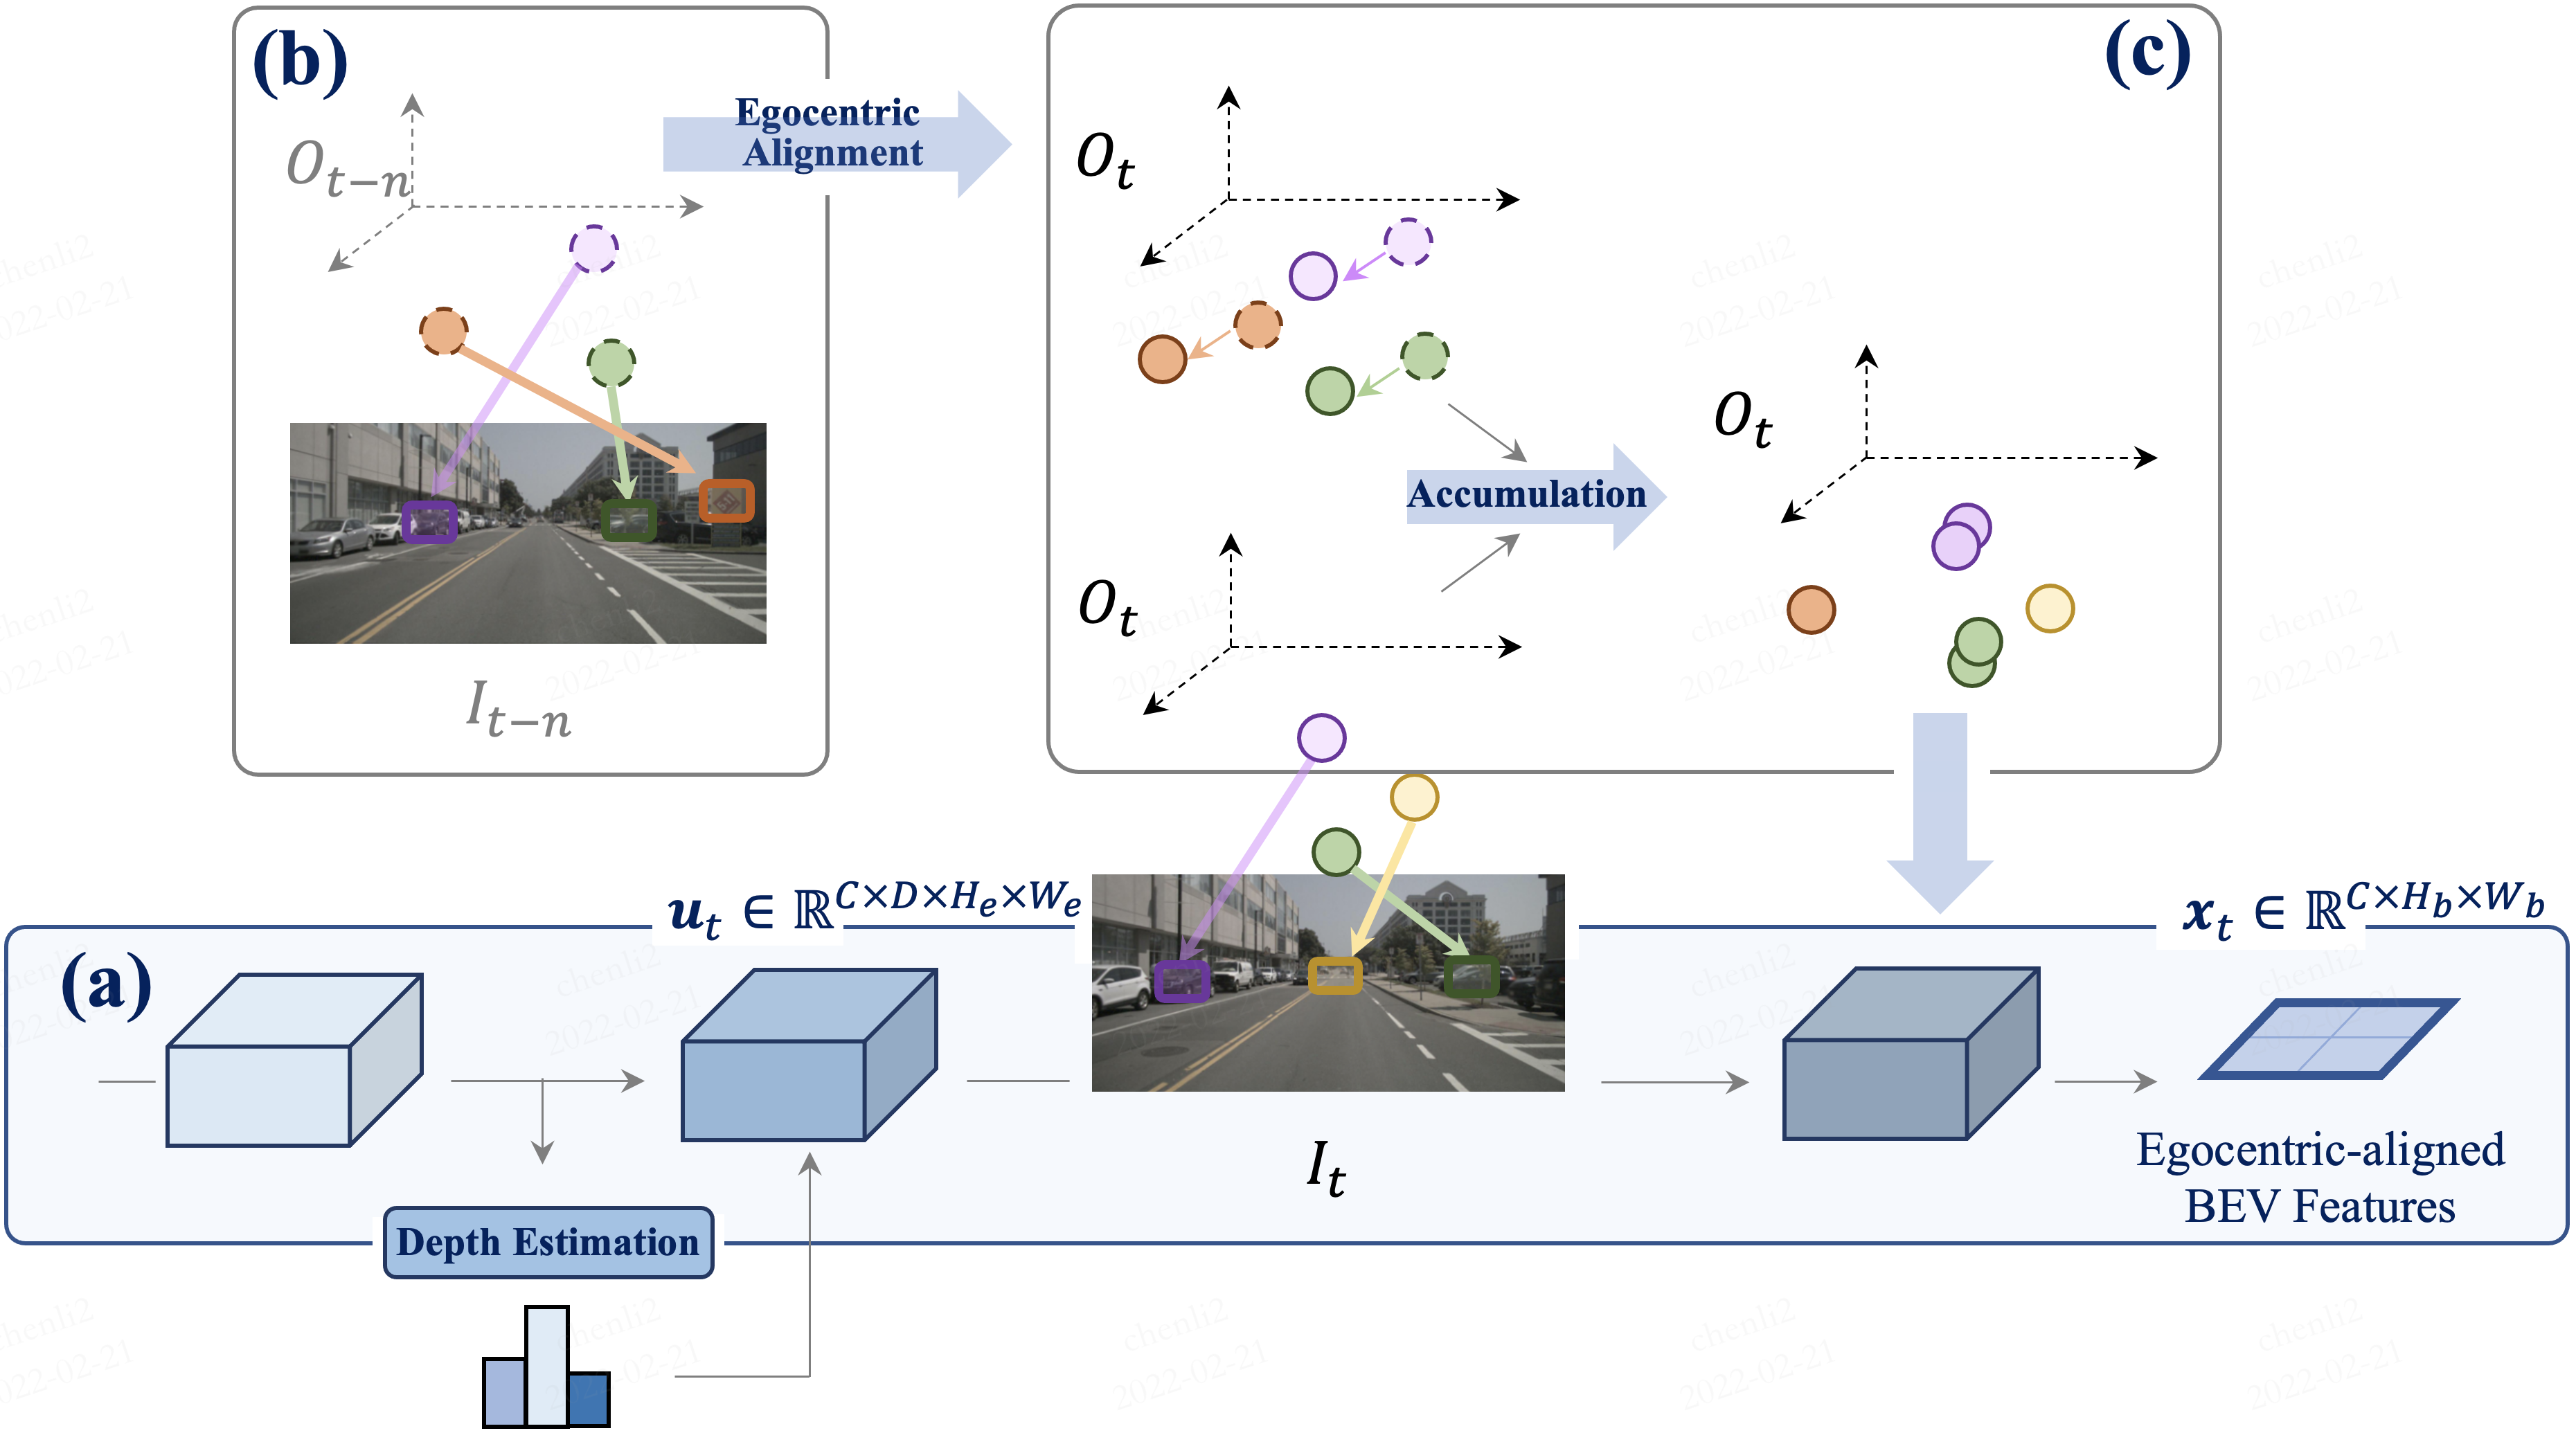
\includegraphics[width=\textwidth]{Figs/perception.png}
    \end{minipage} ~~ % HY: controls lateral space
    \begin{minipage}[b]{0.37\textwidth}
      \caption{
      感知模块的自我中心对齐累积。\textbf{(a)} 当前时间戳的特征通过深度估计提升至 3D，对齐后池化为 BEV 特征 $x_t$；
      \textbf{(b-c)}
      先前帧的 3D 特征对齐到当前视图并与所有过去和当前状态融合，
      使特征表示得到增强
      }
    \label{fig:perception}
    \end{minipage}
    % \vspace{-.2cm}
\end{figure}

\noindent\textbf{空间融合。}
%
一方面，多视角图像特征需变换到共同坐标系。
%
受\cite{philion2020lift}启发，提取每张图像特征并预测对应深度，然后将其提升至全局 3D 坐标系。
%
具体而言，每张相机图像 $I_t^n \in \mathbb{R}^{3 \times H \times W}$ 通过主干网络获得特征 $f_i^k \in \mathbb{R}^{C \times H_e \times W_e}$ 和
深度估计 $d_i^k \in \mathbb{R}^{D \times H_e \times W_e}$，
%
其中 $i \in \{1,\dots,t\}$，$n \in \{1,\dots,6\}$，$C$ 为特征通道数，$D$ 表示离散深度数量，$(H_e, W_e)$ 表示空间尺寸。
%
%
由于缺乏精确深度信息，通过外积将特征沿整个射线空间根据预测深度分布进行散布：
\begin{equation}
	u_i^k = f_i^k \otimes d_i^k,
\end{equation}
其中 $u_i^k \in \mathbb{R}^{C \times D \times H_e \times W_e}$。
%
然后利用相机外参和内参将相机特征锥体 $u_i \in \{u_i^1,\dots,u_i^n\}$ 变换到全局 3D 坐标系，该坐标系原点位于时间 $i$ 时自车惯性中心。
%

另一方面，空间融合需要将过去特征对齐到当前帧，供后续预测和规划任务使用。
%
利用从时间 $t-1$ 到 $t$ 的自车运动（Ego-motion），可将时间 $t-1$ 获取的立方体变换到以时间 $t$ 时 SDV 为中心的坐标系。
%
相同过程可应用于过去帧，从而得到所有过去时间戳的自车中心特征 $\{u_i^{'}\}$。
%
最终，BEV 特征图 $b_i \in \mathbb{R}^{C \times H_b \times W_b}$ 可通过沿垂直维度求和池化从 $\{u_i^{'}\}$ 得到。

\noindent\textbf{时间融合。}
%
经典时间融合方法直接对堆叠的 BEV 特征使用 3D 卷积。
%
但值得注意的是，若某物体在地面上是静止的（如车道线和静态车辆），则不同立方体中相同位置对应的特征应相似。
%
利用这一特性，
可通过将先前 BEV 特征图加到当前特征图来执行自注意力增强静态物体感知能力，公式如下（折扣系数 $\alpha = 0.5$，$\tilde{x}_1 = b_1$）：
%
\begin{equation}
\tilde{x}_t = b_t + \sum_{i=1}^{t-1} \alpha^i \times \tilde{x}_{t-i},
\end{equation}

为更精确感知动态物体，将这些特征馈入由 3D 卷积实现的时间融合网络。为补偿自车运动引起的偏差，将运动矩阵通过空间通道拼接方式加入特征：
\begin{equation}
    x_{1\sim t} = \mathcal{C}(\tilde{x}_{1 \sim t}, m_{1 \sim t}),
\end{equation}
其中 $m_{1 \sim t}$ 表示自车运动矩阵，$\mathcal{C}$ 表示 3D 卷积网络。

%\{temporal model can be said that it can self-attention the dynamic object compared to the above static object. Need the experiments to stand up. \}






\subsection{预测：双路径概率未来建模}\label{sec: method-prediction}

在动态驾驶环境中，传统运动预测算法\cite{wu2020motionnet,fang2020tpnet,djuric2020uncertainty}通常将未来轨迹预测为确定性或多模态结果。
%
然而，由于智能体之间、交通元素与道路环境之间的交互，有限数量的概率建模无法覆盖未来的复杂情况。
%
为应对未来的随机性，希望在预测特征中推理条件不确定性。
%
受 Hu \textit{et al}.~\cite{hu2020probabilistic} 启发，将未来不确定性建模为对角高斯分布（Gaussian distribution），包含均值 $\mu \in \mathbb{R}^L$ 和方差 $\sigma^2 \in \mathbb{R}^L$，其中 $L$ 为隐通道数。
%
从分布中采样的样本可作为供未来使用的隐状态特征。
%
注意训练时使用采样 $\eta_t \sim \mathcal{N}(\mu_{\mathrm{t}}, \sigma^2_{\mathrm{t}})$，推理时则从 $\eta_t \sim \mathcal{N}(\mu_{\mathrm{t}}, 0)$ 采样。
%

\begin{figure}[t]
    \centering
    \begin{minipage}[b]{0.59\textwidth}
      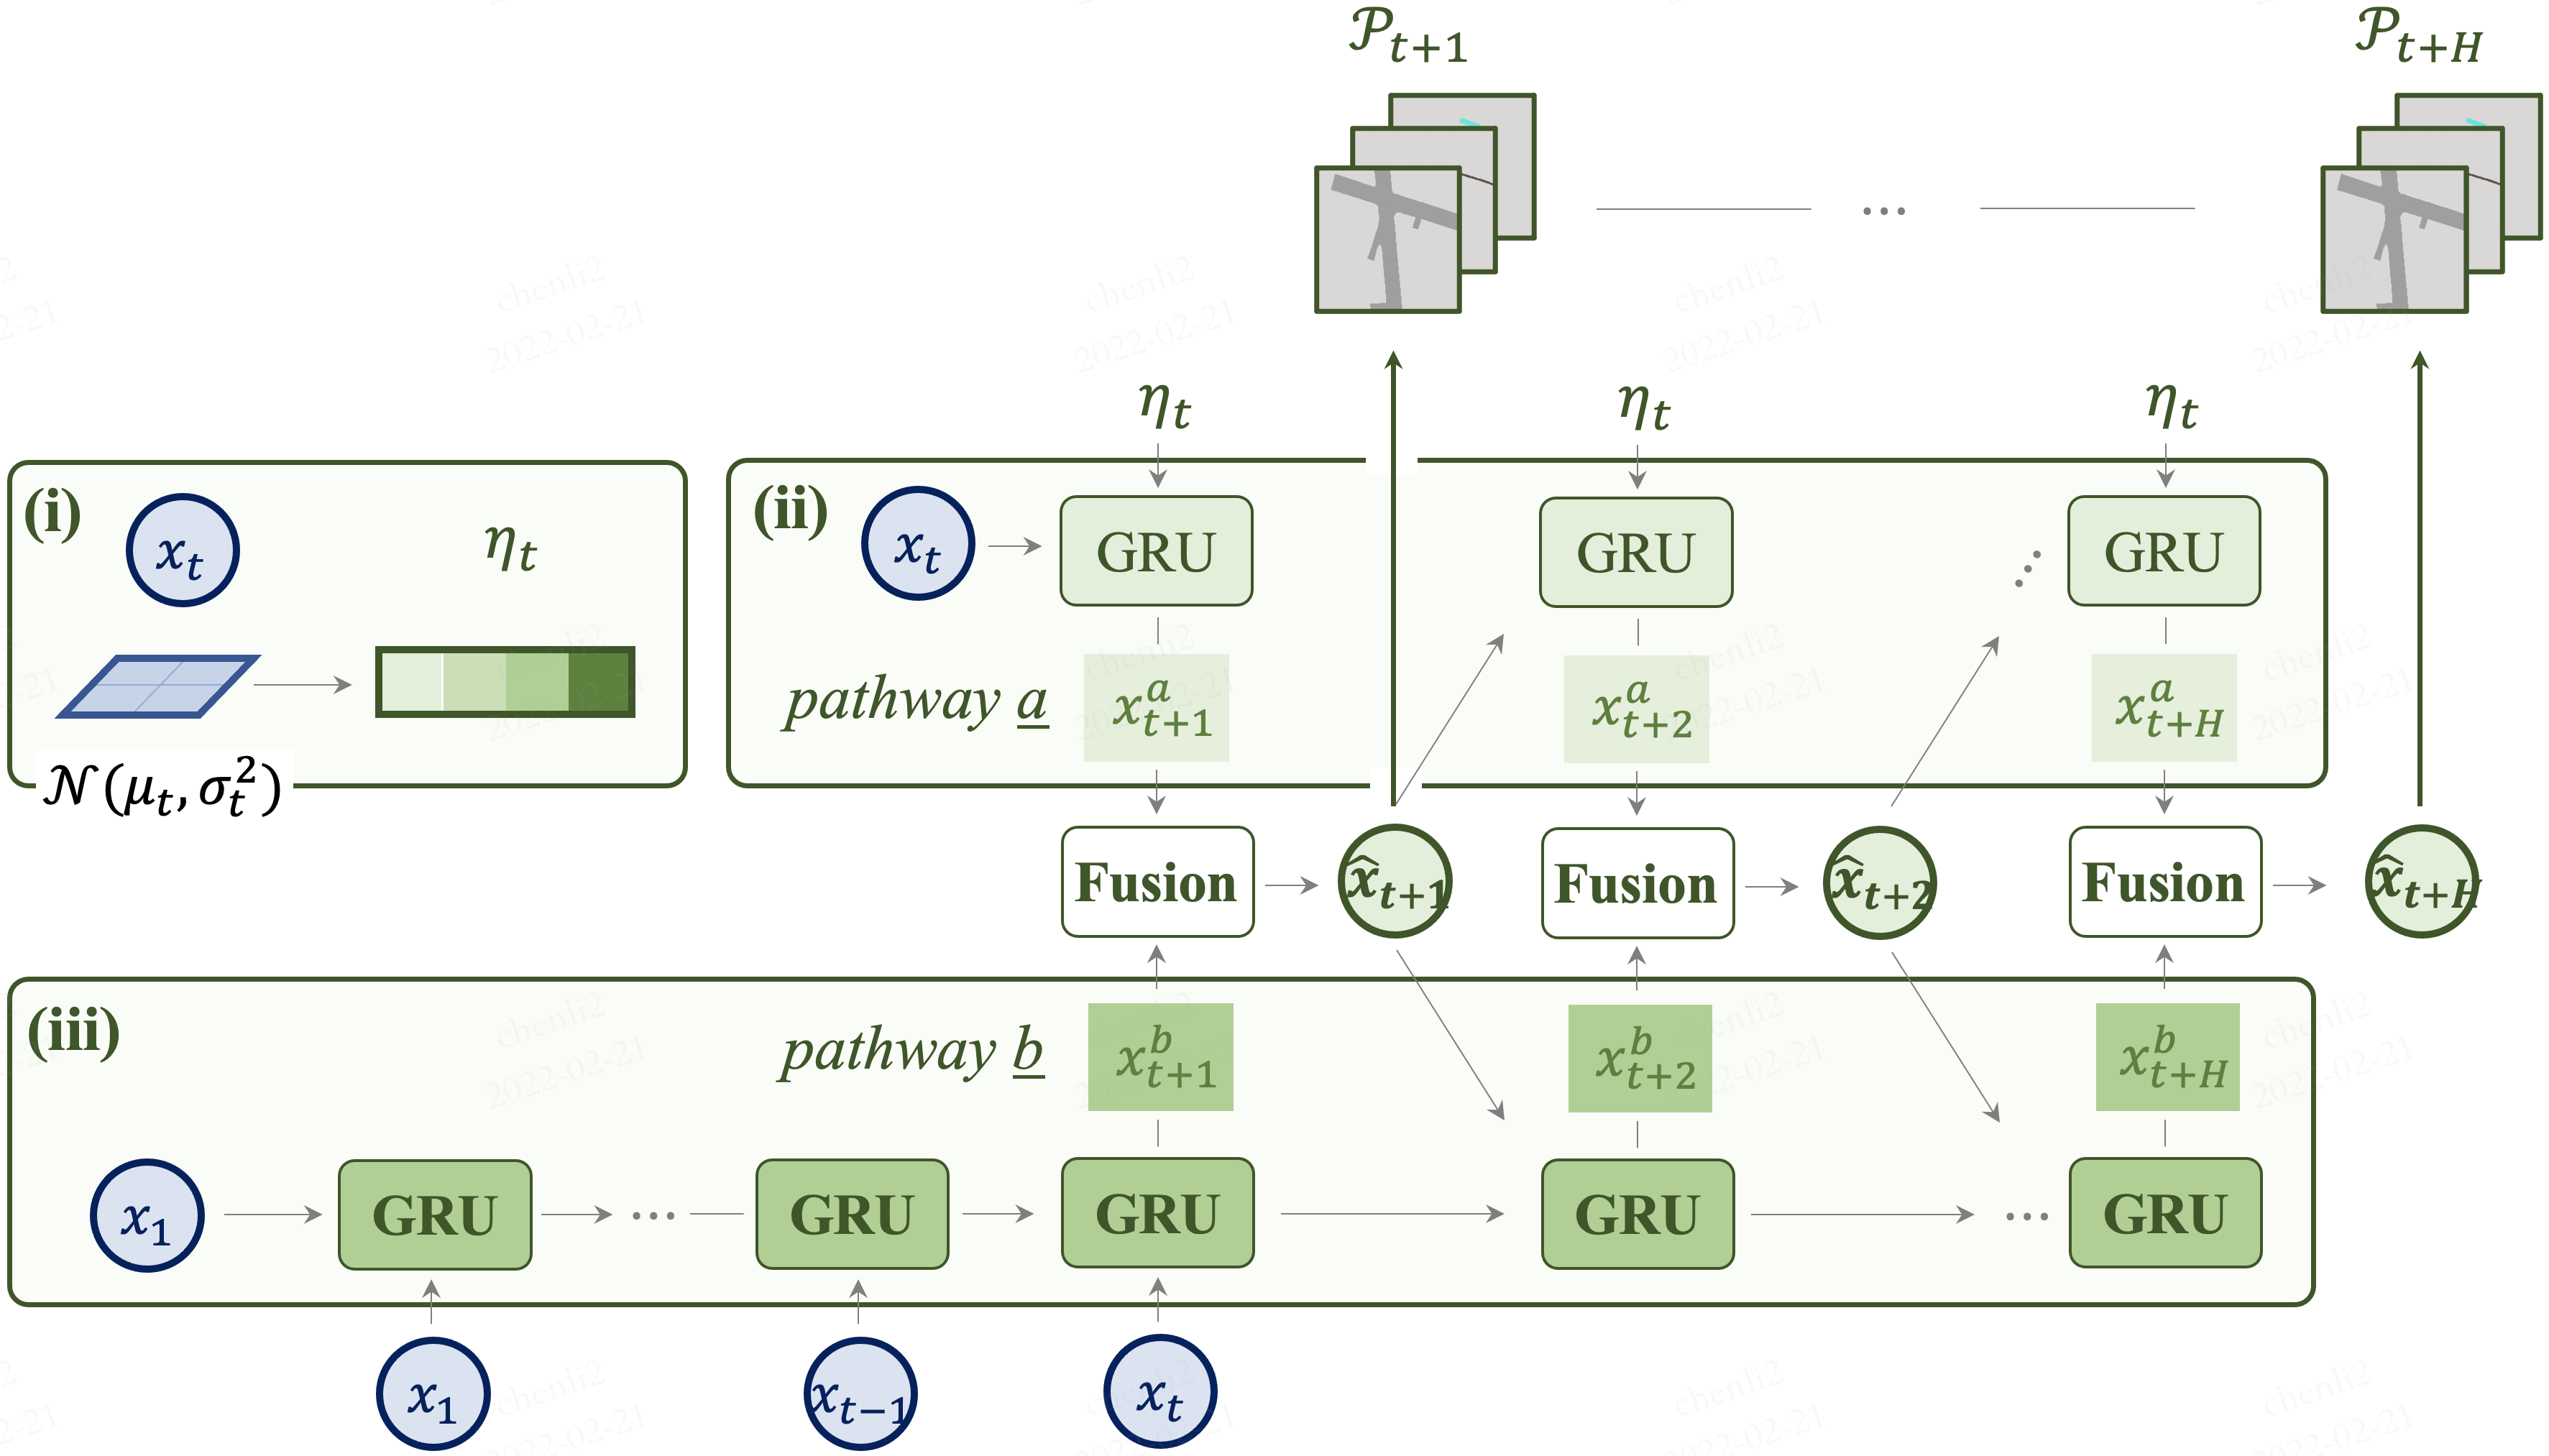
\includegraphics[width=\textwidth]{Figs/prediction.png}
    \end{minipage} ~~ % HY: controls lateral space
    \begin{minipage}[b]{0.37\textwidth}
      \caption{
    %   The detailed network structure of 
      预测模块的双路径建模（Dual Pathway Modelling）。
      %
      \textbf{(i)} 隐码来自特征图分布；\textbf{(ii-iii)}
    %   in ST-P3. 
      路径 \underline{\textit{a}} 利用不确定性分布表示未来多模态性，
      而  
    %   pathway 
      路径 \underline{\textit{b}} 从过去变化中学习，有助于补偿 \underline{\textit{a}} 中信息
    %   An attention-based module is adopted to fuse two predictions
      }
    \label{fig:prediction}
    \end{minipage}
    % \vspace{-.2cm}
\end{figure}


% \begin{figure}[t]
%   \centering
%   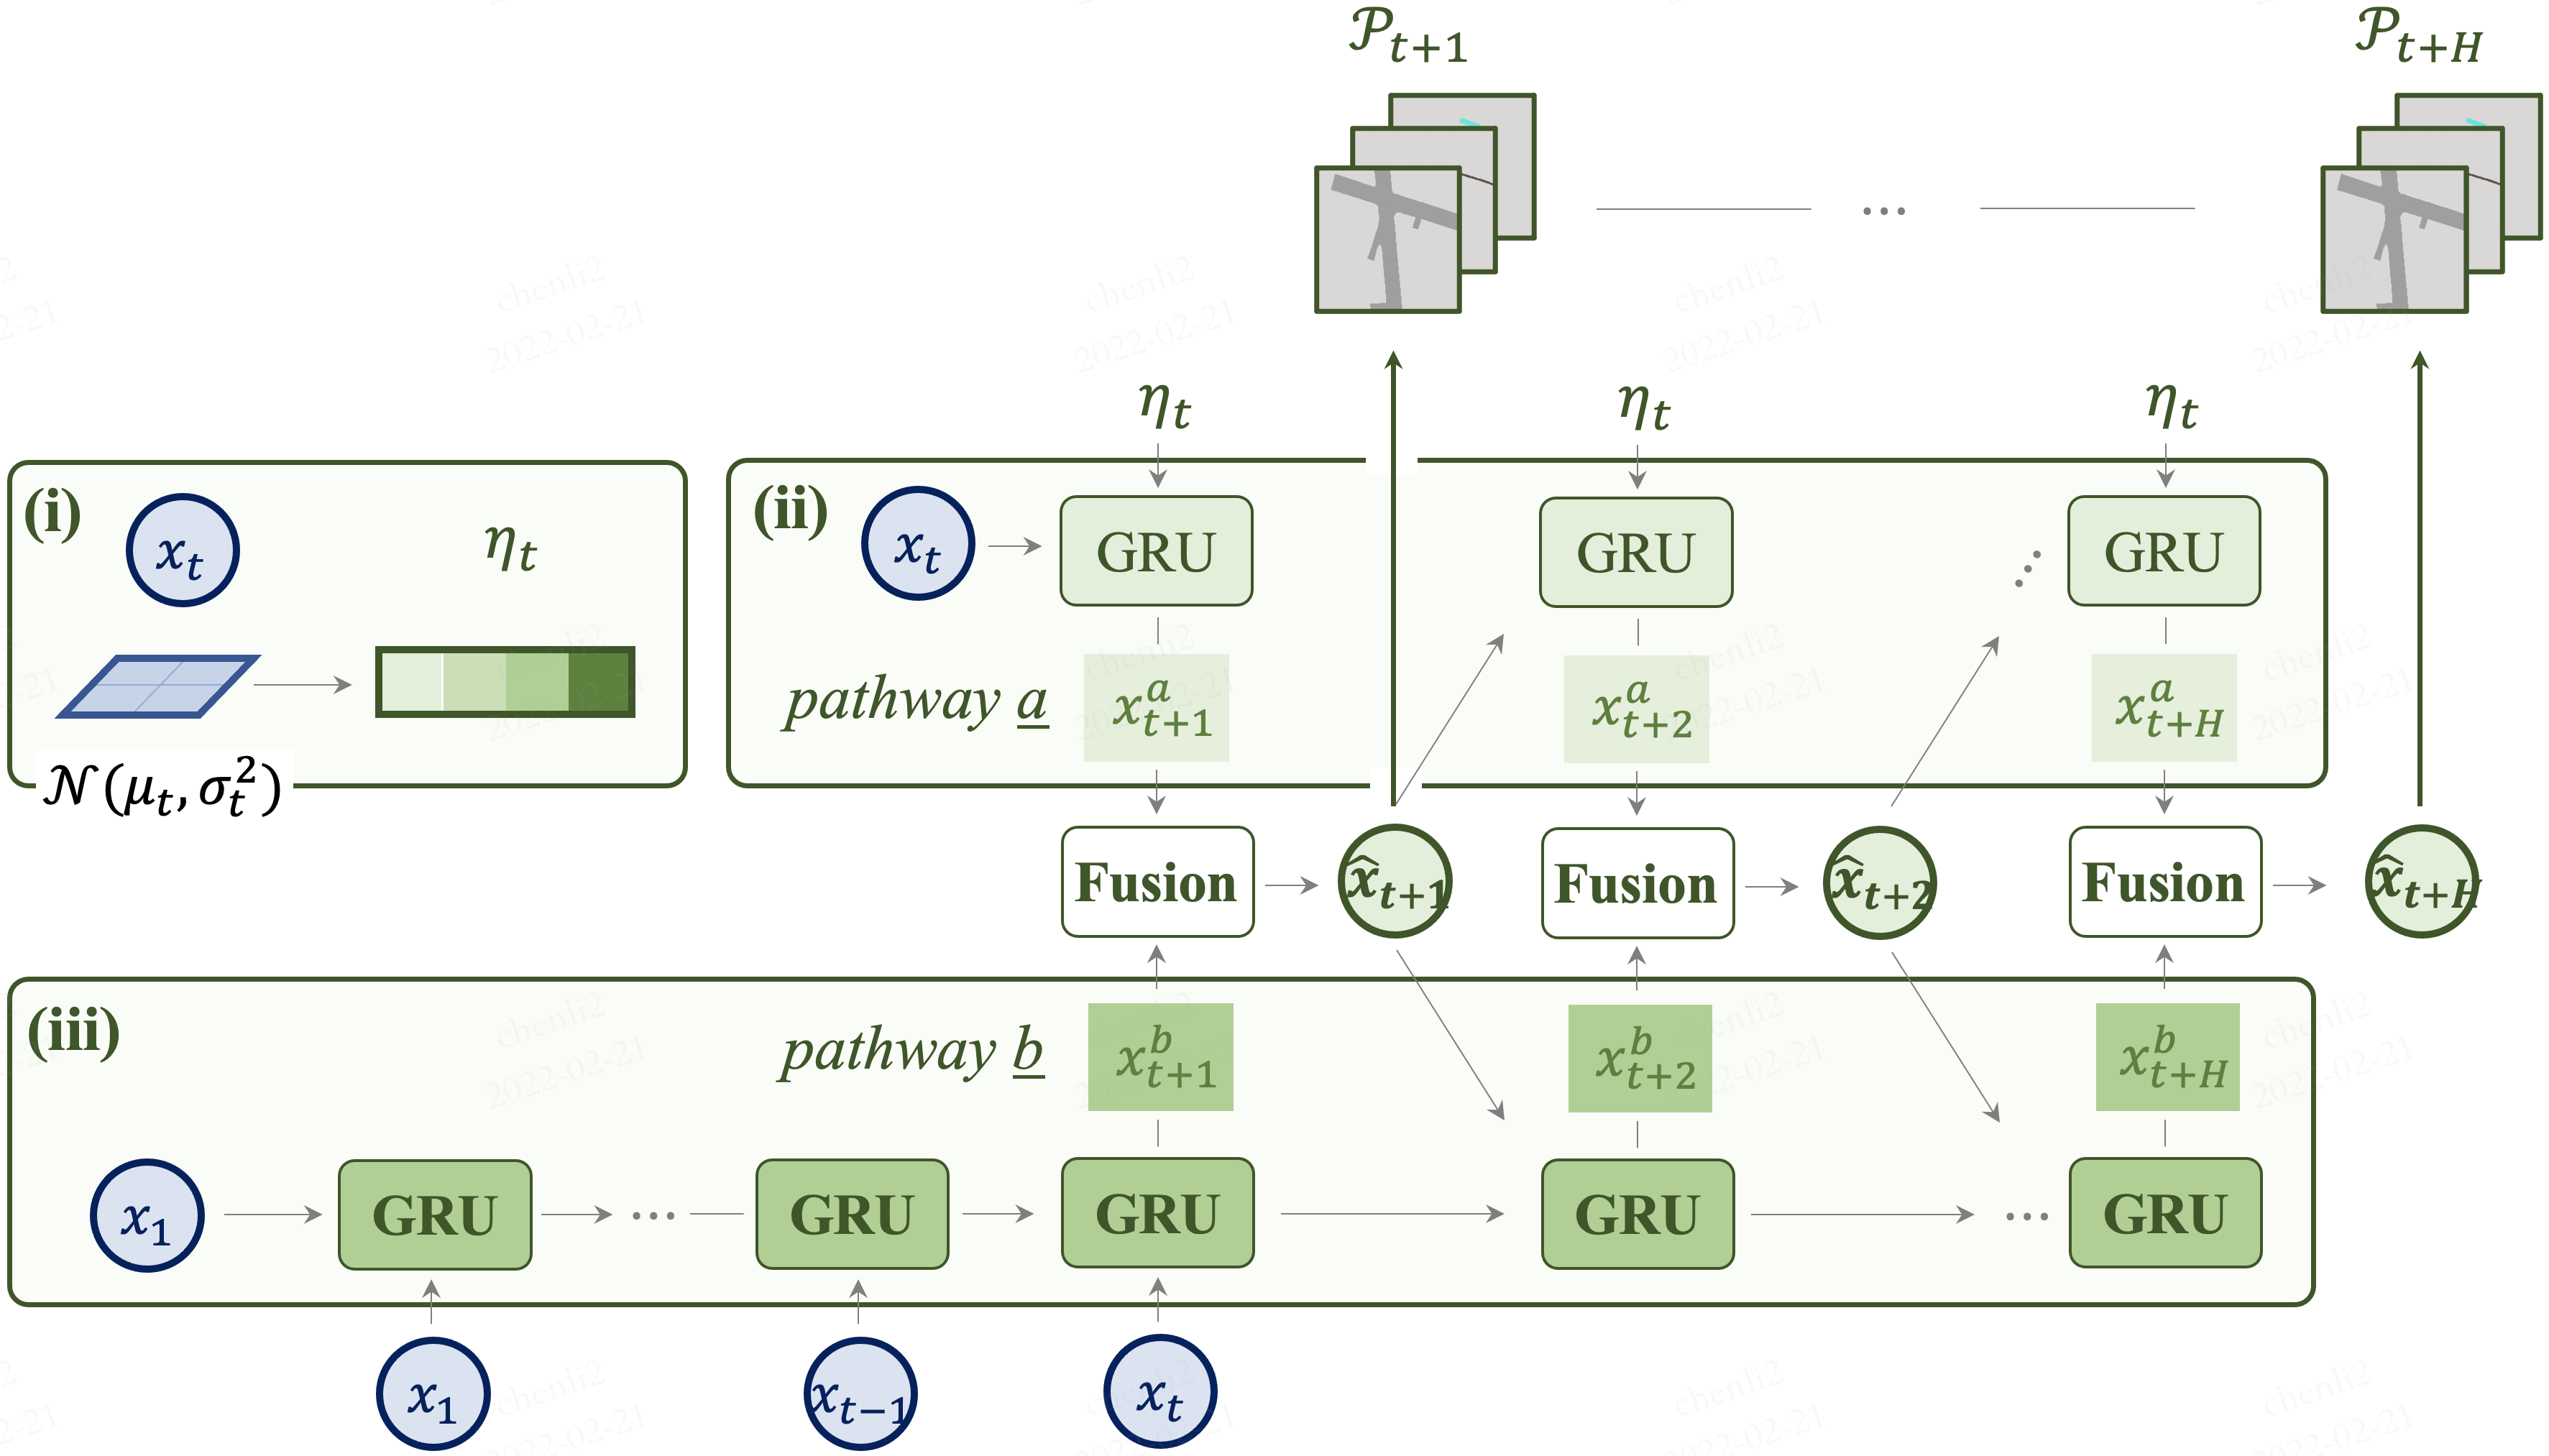
\includegraphics[width=0.6\textwidth]{Figs/prediction.png}
%   \caption{
% %   Prediction, [need embellish]
% The detailed network structure of Dual GRU module in ST-P3. The upper path incorporates the uncertainty distribution to represent the multi-modal of future, while the lower path learns from features in the past. An attention-based Mix Gate is adopted to fuse the two predictions
%   }
%   \label{fig:prediction}
% \end{figure}


% After getting the future uncertainty distribution, we just use it as the hidden state to the prediction module, which is modeled by the convolutional gated recurrent unit network.
%
% \textcolor{red}{Recurrence through convolutions is a natural fit for motion predictions because it takes the advantage of the spatial invariance of the BEV representations, as the laws of physics are mostly consistent across space.} 
%
预测模块架构
%, \textbf{Dual GRU}, 
如图 \ref{fig:prediction} 所示。
%
将截至当前时间戳的 BEV 特征和未来不确定性分布集成到预测模型中，分别对应双路径建模（Dual Pathway Modelling）中的两条路径。
%
% Formally, We make two predictions at the same time.
%
一条路径以历史特征 $(x_1, \dots, x_t)$ 为 GRU（门控循环单元，GRU）输入，$x_1$ 为初始隐状态（Hidden state）进行预测。另一条路径以 $\eta_t$ 的样本为 GRU 输入，$x_t$ 为初始隐状态。
%
预测时间 $t+1$ 的特征时，以混合高斯形式组合预测特征：
\begin{equation}
    \hat{x}_{t+1} = \mathcal{G}(x_t, \eta_t) \oplus \mathcal{G}(x_{0:t}),
\end{equation}
%
其中 $\mathcal{G}$ 表示 GRU 过程。
%
以混合预测作为后续预测过程的基础。
%
通过此方法，双路径建模递归地预测未来状态 $(\hat{x}_{t+1},\dots, \hat{x}_{t+H})$。



% Finally, 
所有特征 $(x_1, \dots, x_t), (\hat{x}_{t+1},\dots, \hat{x}_{t+H})$ 馈入解码器（Decoder）$\mathcal{D}$，该解码器含多个输出头，生成不同的可解释中间表示。
%
结果见图 \ref{fig:pred outputs}。
%
对于实例分割（Instance segmentation）任务，遵循~\cite{hu2021fiery} 的评估指标，输出头生成实例中心度、偏移和未来光流。
%
同时，语义分割（Semantic segmentation）头主要关注车辆和行人，这两个是驾驶场景中的主要智能体（Agent）。
%
此外，由于 HD map 在自动驾驶中扮演重要角色~\cite{sadat2020perceive,sadat2019jointly,zeng2019end}，显式生成两个元素——可行驶区域和车道线，以提供可解释的地图表示。
%
代价体（Cost volume）头设计用于表示 SDV 在规划范围内每个可能位置的\textit{代价}。代价体更多细节见第 \ref{sec: method-plan} 节。
%
注意，也对过去帧特征进行解码以提升历史特征精度，这是双路径建模所需要的。如第 \ref{sec: res-nuscenes} 节所示，更精确的特征信息可带来更好的预测。
% effect.






\subsection{规划：先验知识融合与优化}
\label{sec: method-plan}

% \begin{figure}[tb!]
%   \centering
%   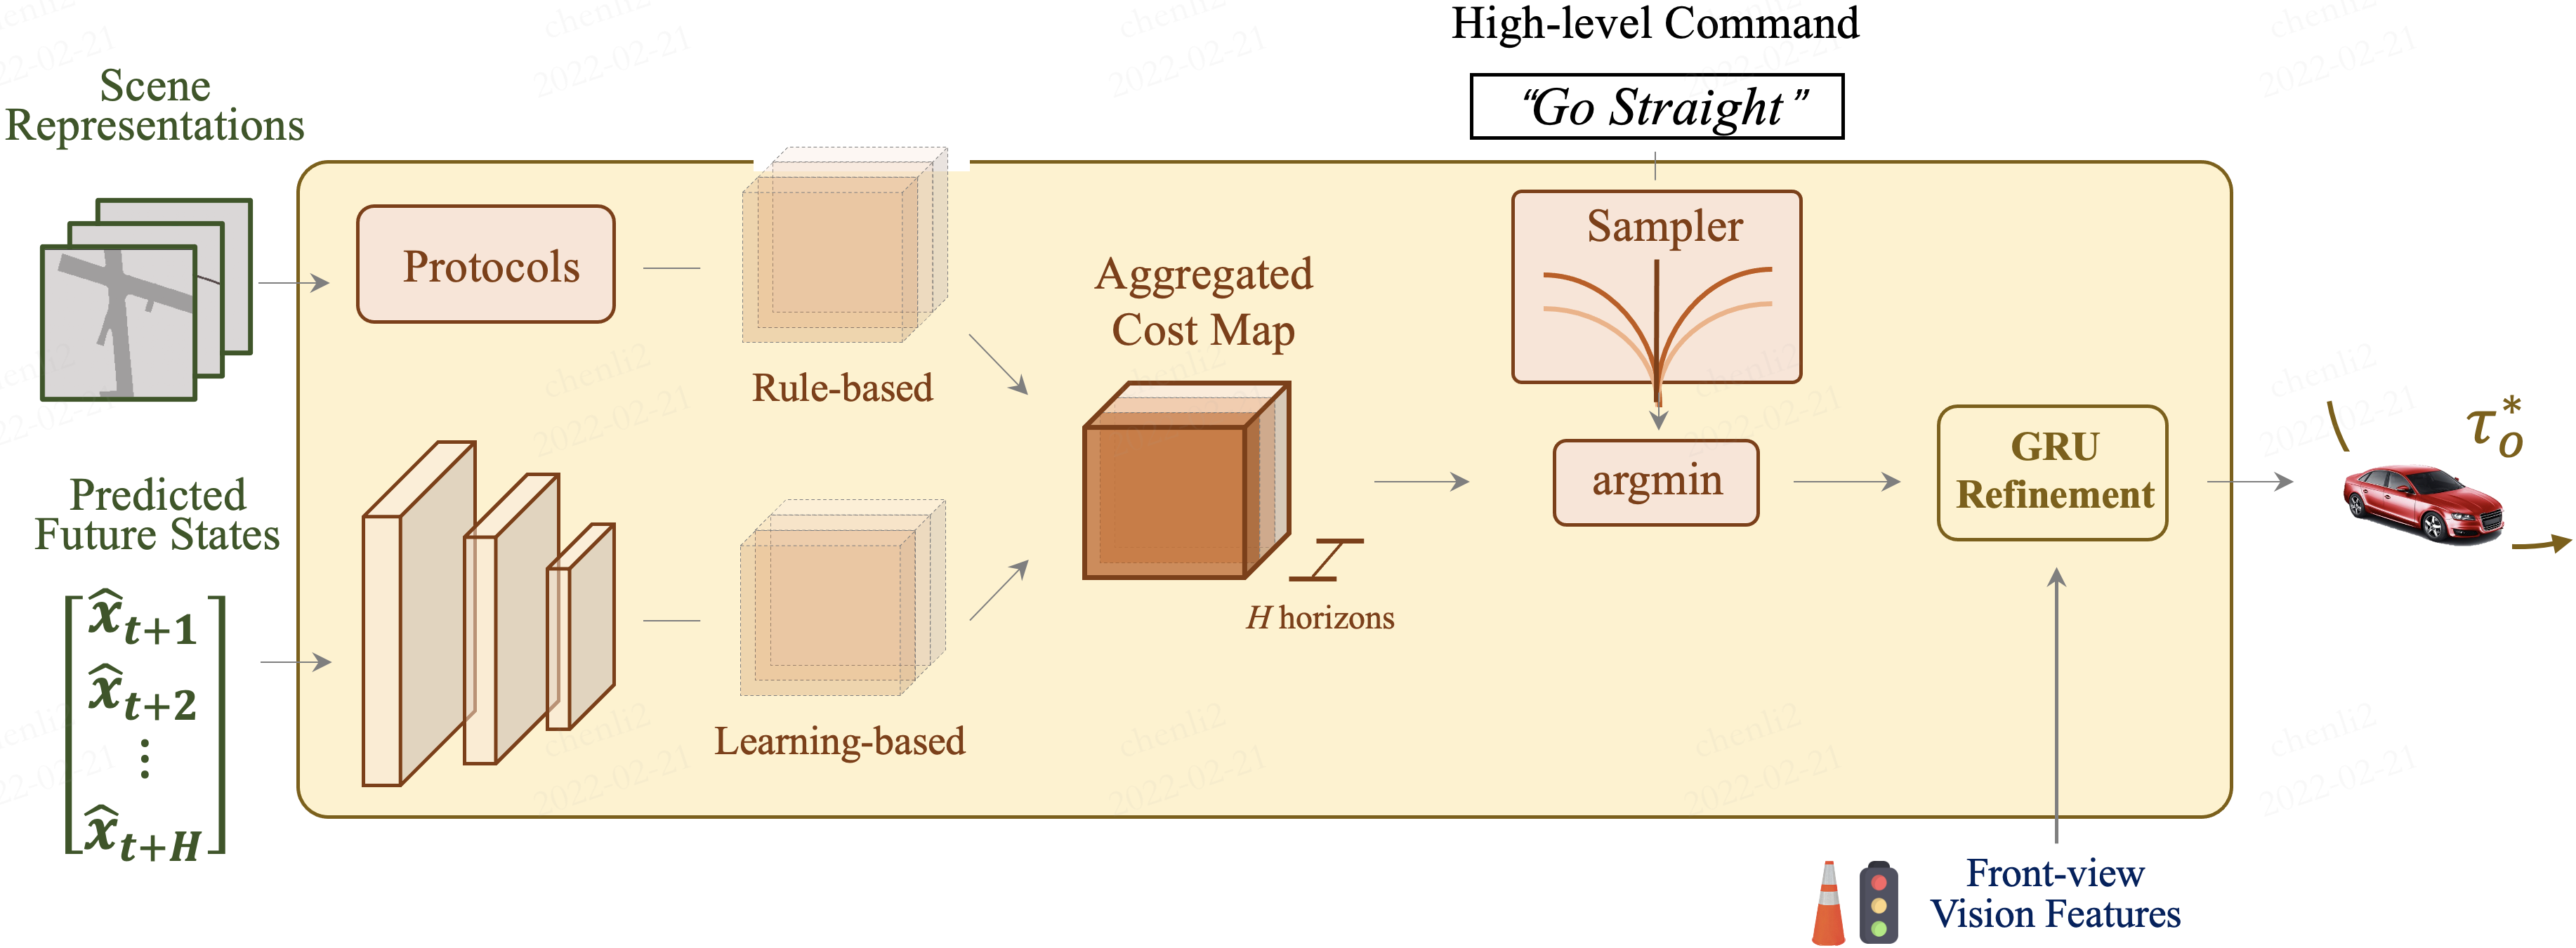
\includegraphics[width=0.6\textwidth]{Figs/planning.png}
%   \caption{规划模块的详细架构}
%   \label{fig:planning}
% \end{figure}

\begin{figure}[t]
    \centering
    \begin{minipage}[b]{0.6\textwidth}
      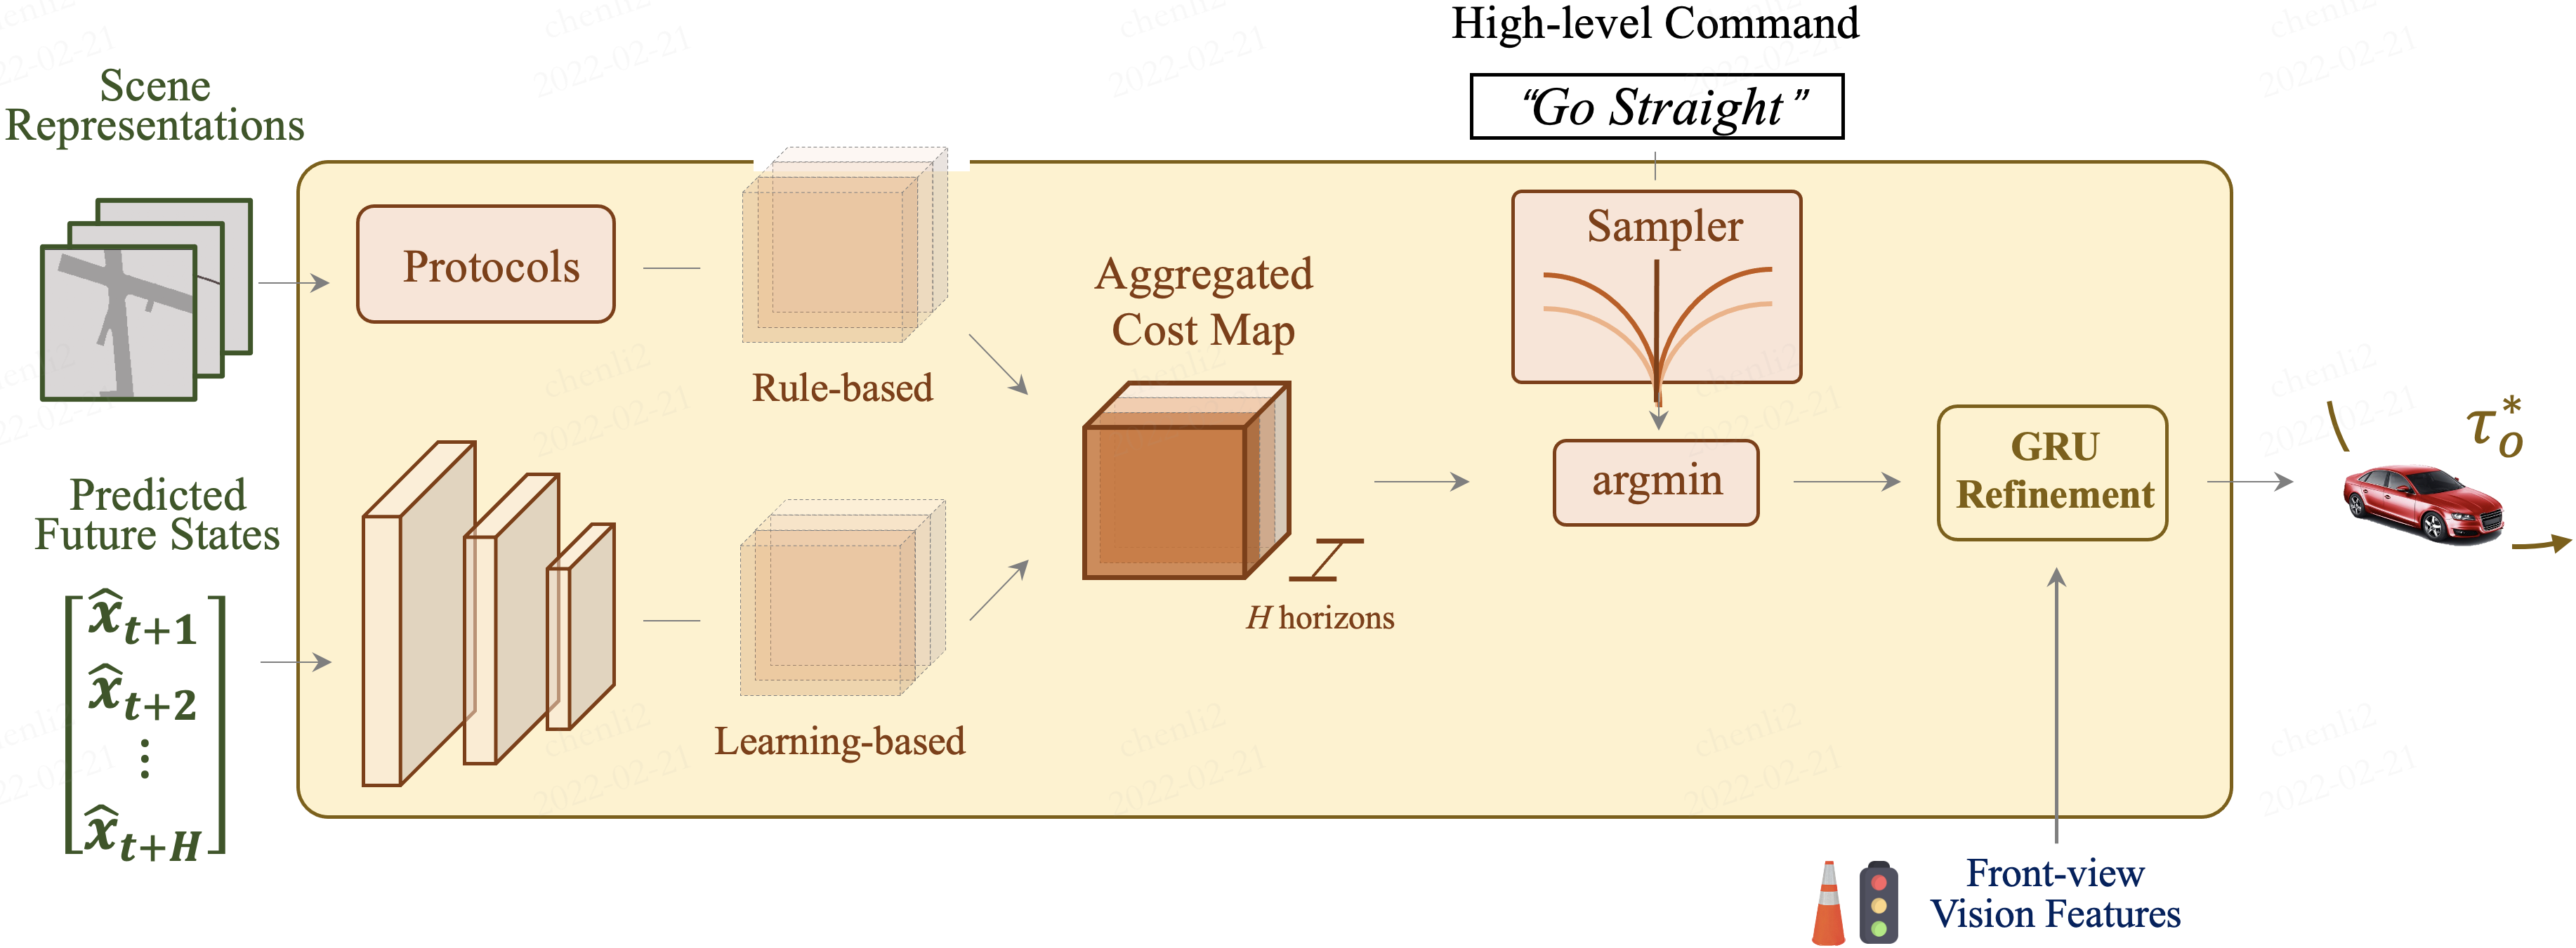
\includegraphics[width=\textwidth]{Figs/planning.png}
    \end{minipage}  % HY: controls lateral space
    \begin{minipage}[b]{0.37\textwidth}
      \caption{
      规划模块的先验知识融合与优化（Prior Knowledge Incorporation and Refinement）。 
    %   Detailed architecture of the planning module. 
      整体代价图（Cost map）包含两个子代价。 
      最小代价轨迹进一步通过前视图特征优化，以聚合来自相机输入的视觉信息
      }
    \label{fig:planning}
    \end{minipage}
\end{figure}

作为最终目标，运动规划器需规划一条安全舒适的轨迹到达目标点。
%
给定占用预测 $o$ 和地图表示感知 $m$，本文设计运动规划器——采样多样化轨迹集，选择使学习到的代价函数最小化的轨迹，受~\cite{zeng2019end,sadat2020perceive,casas2021mp3} 启发。
%
但本文与之不同处在于，利用时序模型增加额外优化步骤，集成目标点和交通灯信息。
%
整体模块如图 \ref{fig:planning} 所示。

代价函数充分利用学习到的占用概率场（预测模块中的分割图）和丰富先验知识（如交通规则），确保最终轨迹的安全性和平滑性。
%
形式上，给定 SDV 动态状态，采用自行车模型~\cite{polack2017kinematic} 采样轨迹集 $\tau$。
%
%
目标代价函数 $f$ 由子代价组成：$f_o$ 根据先验知识评估每个时间戳 $t$ 的预测轨迹，$f_v$ 来自预测解码器（基于学习），$f_r$ 与轨迹整体表现相关（如舒适性、进度）。
%
因此整体代价函数可表示为等权组合：
\begin{equation}
    f(\tau, o, m; w) = f_o(\tau, o, m; w_o) + f_v(\tau ; w_v) +f_r(\tau; w_r),
\end{equation}
其中 $w = (w_o,w_v,w_r)$ 为所有可学习参数向量。
% for the cost function. 
下面简要描述各子代价，详细内容请参考附录。

\noindent\textbf{安全代价（Safety Cost）。} SDV 不应与道路上其他物体碰撞，规划轨迹时需考虑它们未来运动。
%
规划轨迹不能与其他智能体或道路元素占用的网格重叠，高速运动时需保持一定安全距离。
% Moreover, the SDV usually follows a leading vehicle and needs to keep a certain safe distance from it which mainly depends on the speed of the leading vehicle. Also, it is encouraged that the SDV stays in the middle of the lanes and a cost function is set as the distance to the perceived lanes in the first stage.
%Since we have no HD map information, we manually perceive the lane, but due to the limitation of accuracy, we cannot fully trust the result of the perception. Therefore, in order to adapt to this situation, we only consider the lane lines whose perception results exceed a certain probability. We should stay in the center of the lane line, that is, we should keep a certain distance from the lane line, so our cost function is set so that the closer to the lane line, the greater the cost value.

\noindent\textbf{代价体（Cost Volume）。} 由于道路信息复杂性，无法手动枚举所有可能情况或规划代价，因此引入第 \ref{sec: method-prediction} 节中输出的学习型代价体。
%
为平衡代价尺度，对值进行裁剪，使其不在轨迹评估中占据主导地位。

\noindent\textbf{舒适性与进度（Comfort and Progress）。} 对具有较大横向加速度、加加速度或曲率的轨迹施加惩罚。
%
期望轨迹高效到达目的地，因此正向行进的轨迹获得奖励。



然而，上述代价不包含目标信息——目标信息通常由路由地图提供，但本文设置中不可用。
%
因此采用高层指令（High-level command），包括前进、左转和右转，仅根据对应指令评估轨迹。
%
% and the long-distance target point.
%
% The information is similar to the lane level information as the GPS provides to human drivers.
%
% For efficient use of this, we only evaluate the trajectories which belong to the command.
%
总结而言，运动规划器输出代价最小的轨迹：
\begin{equation}
    \tau^* = \arg\min_{\tau_h} f(\tau_h, c) = \arg\min_{\tau_h} f(\tau_h, o, m; w), 
    \label{eq:over_obj}
\end{equation}
其中 $\tau^*$ 为选中轨迹，$\tau_h$ 为对应高层指令下的轨迹集，$c$ 为整体代价图。
%
%
此外，交通灯对 SDV 至关重要，但之前模块未显式利用。通过 GRU 网络将交通灯信息纳入轨迹优化。
%
%
用编码器模块的前视相机特征初始化隐状态（Hidden state），以 $\tau^*$ 中每个采样点为输入。
%
%
表 \ref{tab:p2_ablation} 表明前视相机特征确实捕捉了交通灯信息，帮助 SDV 在交叉口启停。

\subsection{端到端学习的整体损失
}\label{sec: method-e2e learning}
通过以下损失函数以端到端方式联合优化感知、预测、规划模块：
\begin{equation}
    \mathcal{L} =  \mathcal{L}_{per} + \alpha \mathcal{L}_{pre} + \beta \mathcal{L}_{pla}.
\end{equation}
遵循~\cite{kendall2018multi,chen2018gradnorm} 中的协议，权重 $\alpha$、$\beta$ 是可学习的而非固定的，根据对应任务损失的梯度平衡不同任务间尺度。
%$(\omega_{per}, \omega_{pre}, \omega_{pla})$

\noindent\textbf{感知损失（Perception Loss）。}
%
该损失包括当前和过去帧的分割损失、地图损失和辅助深度损失。
%
语义分割采用与~\cite{hu2021fiery} 相同的 top-k 交叉熵损失，因为 BEV 图像主要由背景占据。实例分割中，中心度监督采用 $l_2$ 距离损失，偏移和光流任务采用 $l_1$ 距离损失。
%
车道线和可行驶区域预测采用交叉熵损失。
%
%
当前方法\cite{philion2020lift,wang2021learning} 利用下游任务隐式优化深度预测而非直接监督，但该方法受最终损失函数设计影响显著，缺乏清晰可解释性。
%
因此本文预先用其他网络生成深度值，然后用其指导预测。更多细节见附录。

\noindent\textbf{预测损失（Prediction Loss）。}
%
由于预测模块推断未来语义分割和实例分割，采用与感知相同的 top-k 交叉熵损失。但未来时间戳的损失因预测不确定性而指数衰减。

\noindent\textbf{规划损失（Planning Loss）。}
%
规划模块首先根据式 (\ref{eq:over_obj}) 从采样的轨迹集 $\tau$ 中选择\textit{最优}轨迹 $\tau^*$，然后基于 GRU 的网络进一步优化轨迹得到最终输出 $\tau_o^*$。
%
因此规划损失包含两部分：最大间隔损失（以专家行为 $\tau_h$ 为正样本、采样轨迹为负样本）和输出与专家轨迹之间的 $l_1$ 距离损失。具体而言：
\begin{equation}
    \mathcal{L}_{pla} = \max_{\tau} \left[ f(\tau_h, c) - f(\tau, c) + d(\tau_h, \tau) \right]_+ + d(\tau_h, \tau_o^* ),
\end{equation}
其中 $[ \cdot ]_+$ 表示 ReLU，$d$ 为输入轨迹之间的 $l_1$ 距离。 

%We use the uncertainty \{FIERY\} to weight the different tasks in order to balance the losses scale.





% \clearpage
\section{实验}\label{sec: experiments}
% \subsection{Protocols}
在开环（Open-loop）和闭环（Closed-loop）两种环境下评估 ST-P3。 
%
采用 nuScenes 数据集\cite{caesar2020nuscenes} 进行开环评估，CARLA 仿真器\cite{dosovitskiy2017carla} 进行闭环演示。
%
默认取过去 $1.0s$ 上下文，预测未来 $2.0s$ 上下文，对应过去 3 帧和未来 4 帧。协议更多细节见附录。


% \indent\textbf{Dataset.}
% We evaluate ST-P3 in both open-loop and closed-loop environments. 
% %
% We adopt nuScenes dataset~\cite{caesar2020nuscenes} for the open-loop setting,  and CARLA simulator~\cite{dosovitskiy2017carla} for the closed-loop demonstration.

% % \textbf{nuScenes.}
% %
% % nuScenes contains 1000 scenes, each 20 seconds annotated at 2Hz. 
% %The camera setup consists of 6 cameras covering a full $360^{\circ}$ field of view around the SDV, with a small portion of overlap in between.
% %
% %Every camera in every scene comes with its intrinsics and extrinsics as well.
% %
% %In our experiment, 
% For nuScenes, by default we take the $1.0s$ of past context and predict the future $2.0s$ contexts, which corresponds to 3 frames in the past and 4 frames in the future.
% %
% Since each batch input to the model contains 7 frames of contexts, we just follow the offical split method to split the dataset into training, validation that consist of 26124 and 5719 samples, respectively.
% %
% % For a fair comparison with other BEV representation methods, the BEV spatial is $(100m, 100m)$ around the SDV with resolution $(0.50m,0.50m)$, following the setting in~\cite{hu2021fiery}.

% % \textbf{CARLA.}
% %
% For CARLA, 
% % is a simulation environment where 
% we conduct closed-loop evaluation. Note that we still need to train our model in a open-loop manner first.
% %
% We follow the dataset collection in~\cite{prakash2021multi} and use the Town05 scenario for evaluation and the rest for training. 
% %
% %We collect the driving dataset in different scenes, weather and illumination conditions according to~\cite{prakash2021multi}.
% %
% %Since CARLA 0.9.10 consists of 8 publicly available towns, Town05 is used as the evaluation and the rest is used for training. We mainly evaluate our model in two settings: (1) Town05 Short, (2) Town05 Long.
% %
% %Each route consists of a high density of dynamic agents and adversarial scenarios, which are generated at predefined locations along the route.
% %
% It is worth mentioning that  the camera setup in CARLA only consists of 4 cameras; thus it could not cover the $360^{\circ}$ field of view around the SDV.
% %
% The context from the past 1.0$s$ and current 4 cameras images are passed to our model, then a trajectory is produced and executed by the simulator until SDV getting to the destination or surpassing the time limitation.
% % The temporal setting is same as in nuScenes, but the spatial setting is $(40m, 40m)$ around SDV with resolution $(0.20m, 0.20m)$.


% \noindent\textbf{Implementation Details.}
% We adopt EfficientNet-B4~\cite{tan2019efficientnet} as the backbone, and detailed model description would be illustrated in the Supplementary. We use the Adam optimizer with a constant learning rate $2 \times 10^{-4}$. We train our model on 4 Tesla V100 GPUs for 20 epochs at mixed precision.
% %
% The BEV spatial is $(100m, 100m)$ around the SDV with resolution $(0.50m,0.50m)$ on nuScenes dataset, following the setting in~\cite{hu2021fiery} for a fair comparison. While on CARLA, it is $(40m, 40m)$ around SDV with resolution $(0.20m, 0.20m)$. The time interval between two consecutive frames is 0.5$s$ for both datasets.


\begin{figure}[tb!]
    \centering
    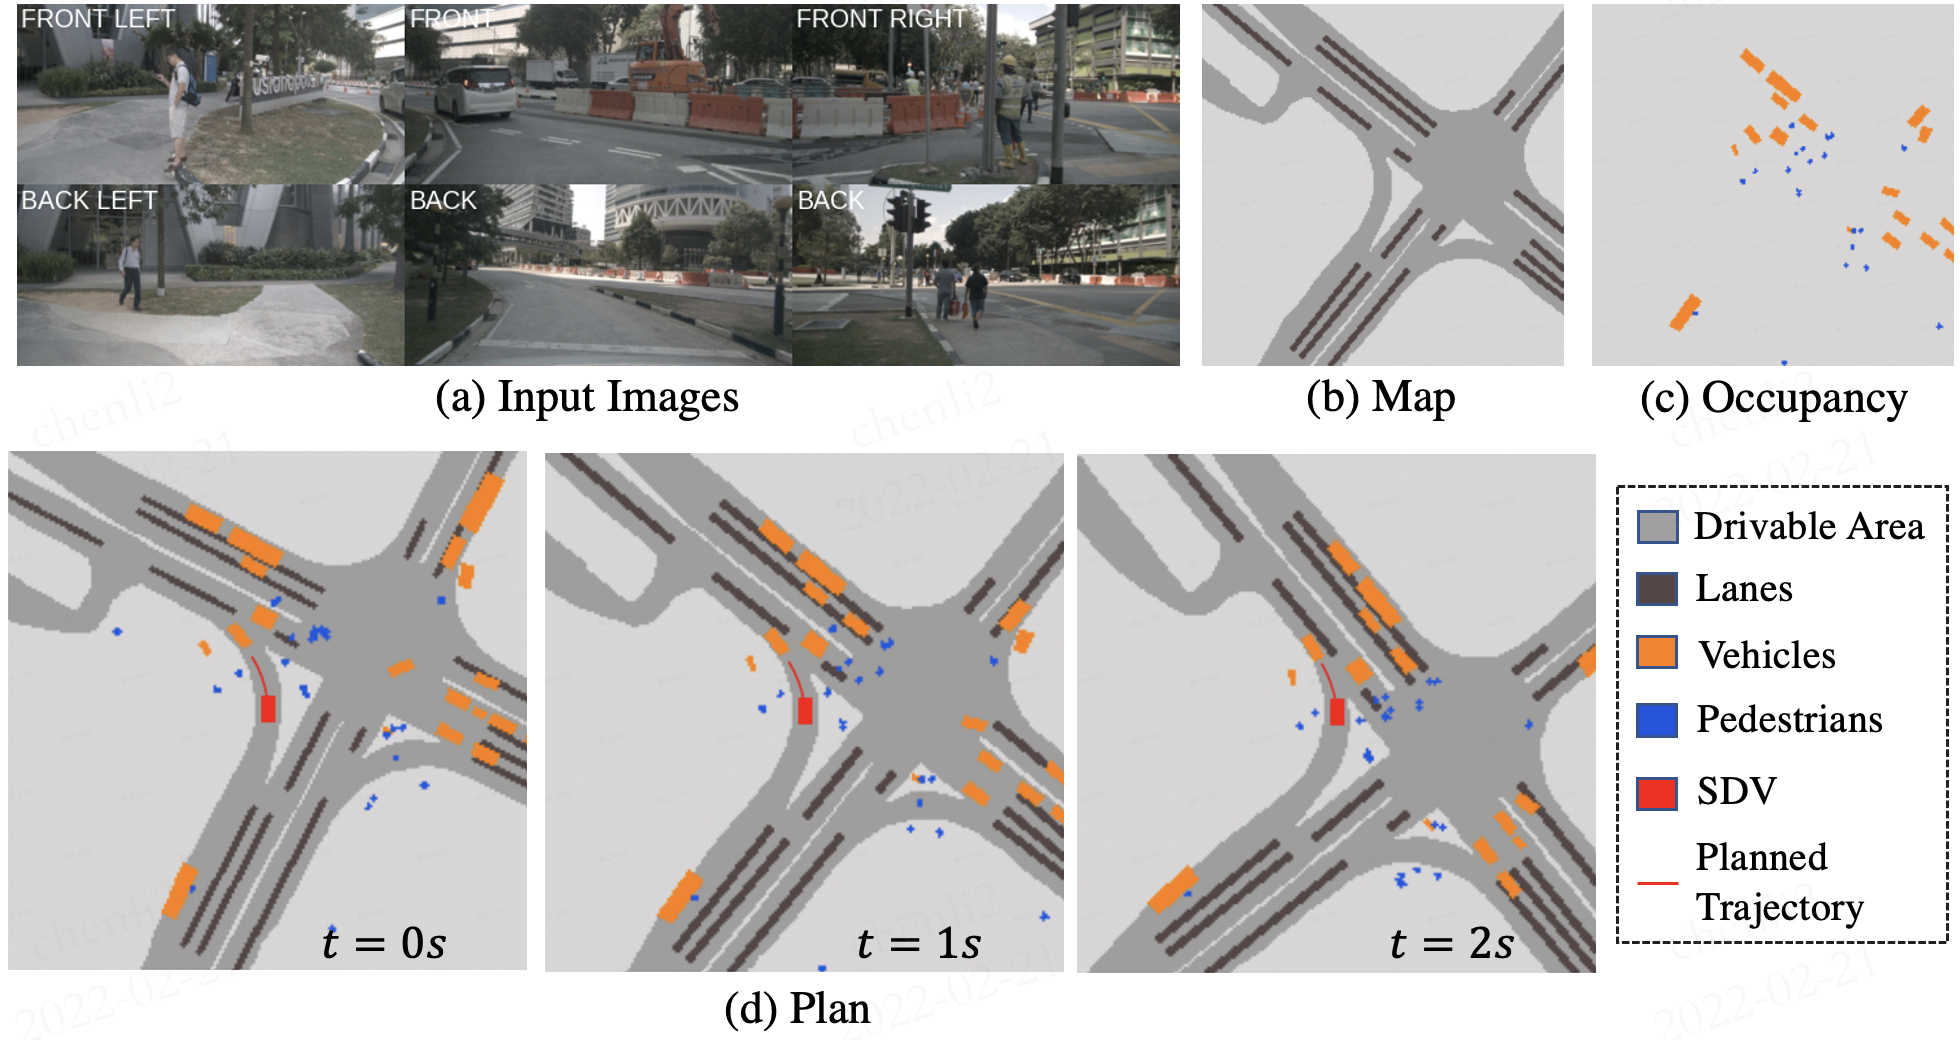
\includegraphics[width=\textwidth]{Figs/output.png}
    \caption{nuScenes 上的定性结果。 (b) 显示预测的地图表示，包括可行驶区域和车道线。 (c) 描绘车辆和行人的分割。 (a-c) 为 $t=1s$ 时刻。 (d) 展示本文模型的整体结果——感知、预测、规划。中间场景表示在时间段内稳健，SDV 成功生成安全轨迹执行左转，未与路缘或前车碰撞
    }
    \label{fig:pred outputs}
    % \vspace{-.3cm}
\end{figure}

\subsection{nuScenes 开环实验结果}\label{sec: res-nuscenes}

% \begin{table}[tb!]
% \caption{Perception results}
% \label{tab:perception}
% \centering
% \scalebox{0.8}{
% \begin{tabular}{p{0.2\textwidth}|>{\centering}p{0.12\textwidth}>{\centering}p{0.12\textwidth}>{\centering}p{0.12\textwidth}>{\centering}p{0.12\textwidth}>{\centering\arraybackslash}p{0.12\textwidth}}
% \toprule
% \multirow{2}{*}{Method}   & Drivable Area     & \multirow{2}{*}{Lane}     & \multirow{2}{*}{Vehicle}     & \multirow{2}{*}{Pedestrian}     & Mean Value     \\ \midrule
% VED~\cite{lu2019monocular}        & 60.82 & 16.74 & 23.28 & 11.93 & 28.19 \\
% VPN~\cite{9123682}                         & 65.97 & 17.05 & 28.17 & 10.26 & 30.36 \\
% PON~\cite{roddick2020predicting}        & 63.05 & 17.19 & 27.91 & 13.93 & 30.52 \\
% Lift-Splat~\cite{philion2020lift} & 72.23 & 19.98 & 31.22 & 15.02 & 34.61 \\
% IVMP~\cite{wang2021learning}       & 74.70  & 20.94 & 34.03 & \textbf{17.38} & 36.76 \\
% FIERY~\cite{hu2021fiery}      & 71.97 & 33.58 & 38.00 & 17.15 & 40.18 \\ \midrule
% \rowcolor{gray!50}
% \textbf{TP3} & \textbf{75.97} & \textbf{40.20} & \textbf{40.10} & 14.48  & \textbf{42.69}\\
% % \textbf{TP3}       &73.74       &38.05       & 39.58       &\textbf{18.45}       &42.46       \\ 
% \bottomrule
% \end{tabular}}
% \end{table}



\textbf{感知（Perception）。} 在地图表示和语义分割上评估模型。
%
感知地图包括可行驶区域和车道线——这两个是驾驶行为最关键的元素，因为 SDV 应在可行驶区域内行驶并保持在车道线中心。
%
语义分割（Semantic segmentation）聚焦车辆和行人，二者是驾驶环境中的主要智能体。
%
采用交并比（Intersection-over-Union, IoU）作为指标，将感知模块建模为 BEV 分割任务。
%
如表 \ref{tab:perception} 所示，ST-P3 在 nuScenes 验证集上获得最高平均值，通过自我中心对齐累积算法超越之前最先进方法（SOTA）\textbf{2.51\%}。
%

% \subsection{Prediction on nuScenes}\label{sec: res-pre}


% \begin{table}[tb!]
% \caption{Predition results. We report semantic segmentation IoU (\%) and instance segmentation metrics from video prediction area. The \textit{static} method assumes all obstacles static in the prediction horizon. ``Ber.'' denotes modeling the future uncertainty as Bernoulli distribution, while ``Gaus.'' means Gaussian distribution. ST-P3 achieves best performance on all temporal segmentation metrics}
% \label{tab:prediction}
% \centering
% \vspace{-7pt}
% \scalebox{0.8}{
% \begin{tabular}{p{0.22\textwidth}|>{\centering}p{0.28\textwidth}|>{\centering}p{0.12\textwidth}>{\centering}p{0.12\textwidth}>{\centering\arraybackslash}p{0.12\textwidth}}
% \toprule
% \multicolumn{1}{l|}{\multirow{2}{*}{Method}} & Future Semantic Seg. & \multicolumn{3}{c}{Future Instance Seg.} \\
% \multicolumn{1}{c|}{}                          & IoU $\uparrow$             & PQ $\uparrow$           & SQ $\uparrow$          & RQ $\uparrow$          \\ \midrule
% Static                                         & 32.20            &    27.64          &   70.72          &   39.08          \\
% FIERY~\cite{hu2021fiery}      & 37.00                                      & 30.20         & 70.20        & 42.90        \\ \midrule
% % \rowcolor{gray!30}
% \textbf{ST-P3 Ber.}                                  & \textbf{38.85}                                     & 32.26        & 70.39       & 45.82       \\
% % \rowcolor{gray!50}
% \textbf{ST-P3 Gaus.}                                   & 38.82                                     & \textbf{32.78}        & \textbf{70.78}       & \textbf{46.32}       \\
% \bottomrule
% \end{tabular}}
% \end{table}


\noindent\textbf{预测（Prediction）。} 在 BEV 中预测未来分割首次在~\cite{hu2021fiery} 中提出，因此选为基线。
%
采用 IoU、全景质量（PQ）、识别质量（RQ）和分割质量（SQ）指标进行评估，遵循视频预测领域的指标\cite{kim2020video}。
%
注意本文仅预测过去帧中已出现的车辆——无法从无到有预测。
%
结果见表 \ref{tab:prediction}。由于预测模块的新颖设计，本文模型在\textit{所有}指标上达到最先进水平。
%
虽然高斯分布（Gaus.）版本略差于 Bernoulli分布（Ber.）版本，最终选择高斯版本以节省内存。

% \subsection{Planning on nuScenes}\label{sec: res-plan}

% \begin{table}[tb!]
% \centering
% \caption{Open-loop Planning results. The \textit{vanilla} approach is supervised with ground truth trajectories only. ST-P3 achieves lowest collision rate in all time intervals}
% \label{tab:planning}
% \vspace{-7pt}
% \scalebox{0.8}{
% \begin{tabular}{p{0.22\textwidth}|>{\centering}p{0.1\textwidth}>{\centering}p{0.1\textwidth}>{\centering}p{0.1\textwidth}|>{\centering}p{0.1\textwidth}>{\centering}p{0.1\textwidth}>{\centering\arraybackslash}p{0.1\textwidth}}
% \toprule
% \multirow{2}{*}{Method}                     & \multicolumn{3}{c|}{L2 ($m$) $\downarrow$} & \multicolumn{3}{c}{Collision (\%) $\downarrow$} \\ \cline{2-7} 
%                                              & 1s      & 2s     & 3s     & 1s        & 2s        & 3s        \\ \midrule
% Vanilla                     & \textbf{0.50}    & \textbf{1.25}   & \textbf{2.80}   & 0.68      & 0.98      & 2.76      \\
% NMP~\cite{zeng2019end}      & 0.61    & 1.44   & 3.18   & 0.66      & 0.90      & 2.34       \\
% Freespace~\cite{hu2021safe} & 0.56    & 1.27   & 3.08   & 0.65      & 0.86      & 1.64      \\  \midrule
% % \rowcolor{gray!50}
% \textbf{ST-P3}                & 1.33    & 2.11   & 2.90   & \textbf{0.23}      & \textbf{0.62}      & \textbf{1.27}      \\ \bottomrule
% \end{tabular}}
% \end{table}

\noindent\textbf{规划（Planning）。} 开环规划聚焦两个评估指标：L2 误差和碰撞率（Collision rate），将规划范围调整至 $3.0s$ 以便公平比较。
%
计算规划轨迹与人类驾驶轨迹之间的 L2 误差，
并评估 SDV 与道路上其他智能体碰撞的频率。
%
%
与先前方法的详细比较见表 \ref{tab:planning}。Vanilla 算法因偏离真值轨迹而受惩罚，因此 L2 误差最低，但在所有预测范围内的碰撞率最高。
%
ST-P3 获得最低碰撞率，表明本文规划轨迹具有优越安全性。
%
% We argue that there are multiple ways to get to the target point and the primary consideration should be the safety. 

\begin{table}[tb!]
\caption{\textbf{感知结果。} 报告中间表示的 BEV 分割 IoU (\%) 及其平均值。ST-P3 在大多数情况下表现最优}
\label{tab:perception}
\centering
% \vspace{-5pt}
\scalebox{0.8}{
\begin{tabular}{p{0.2\textwidth}|>{\centering}p{0.12\textwidth}>{\centering}p{0.12\textwidth}>{\centering}p{0.12\textwidth}>{\centering}p{0.12\textwidth}>{\centering\arraybackslash}p{0.12\textwidth}}
\toprule
\multirow{2}{*}{方法}  & \cellcolor{gray!30}平均值 & 可行驶区域     & \multirow{2}{*}{车道线}     & \multirow{2}{*}{车辆}     & \multirow{2}{*}{行人}          \\ \midrule
VED~\cite{lu2019monocular}      & \cellcolor{gray!30}28.19  & 60.82 & 16.74 & 23.28 & 11.93  \\
VPN~\cite{9123682}                       & \cellcolor{gray!30}30.36  & 65.97 & 17.05 & 28.17 & 10.26  \\
PON~\cite{roddick2020predicting}      & \cellcolor{gray!30}30.52  & 63.05 & 17.19 & 27.91 & 13.93  \\
Lift-Splat~\cite{philion2020lift} & \cellcolor{gray!30}34.61 & 72.23 & 19.98 & 31.22 & 15.02  \\
IVMP~\cite{wang2021learning}      & \cellcolor{gray!30}36.76 & 74.70  & 20.94 & 34.03 & \textbf{17.38}  \\
FIERY~\cite{hu2021fiery}    & \cellcolor{gray!30}40.18  & 71.97 & 33.58 & 38.00 & 17.15  \\ \midrule
\textbf{ST-P3} & \cellcolor{gray!30}\textbf{42.69} & \textbf{75.97} & \textbf{40.20} & \textbf{40.10} & 14.48  \\
% \textbf{TP3}       &73.74       &38.05       & 39.58       &\textbf{18.45}       &42.46       \\ 
\bottomrule
\end{tabular}}
\end{table}

\begin{table}[tb!]
\caption{\textbf{预测结果。} 报告语义分割 IoU (\%) 和来自视频预测领域的实例分割指标。\textit{static} 方法假设预测范围内所有障碍物静止。"Ber." 表示将未来不确定性建模为 Bernoulli分布（Bernoulli distribution），"Gaus." 表示高斯分布（Gaussian distribution）。ST-P3 在所有时序分割指标上达到最佳性能}
\label{tab:prediction}
\centering
% \vspace{-5pt}
\scalebox{0.8}{
\begin{tabular}{p{0.2\textwidth}|>{\centering}p{0.28\textwidth}|>{\centering}p{0.12\textwidth}>{\centering}p{0.12\textwidth}>{\centering\arraybackslash}p{0.12\textwidth}}
\toprule
\multicolumn{1}{l|}{\multirow{2}{*}{方法}} & 未来语义分割 & \multicolumn{3}{c}{未来实例分割} \\
\multicolumn{1}{c|}{}                          & IoU $\uparrow$             & PQ $\uparrow$           & SQ $\uparrow$          & RQ $\uparrow$          \\ \midrule
Static                                         & 32.20            &    27.64          &   70.05          &   39.08          \\
FIERY~\cite{hu2021fiery}      & 37.00                                      & 30.20         & 70.20        & 42.90        \\ \midrule
% \rowcolor{gray!30}
% \rowcolor{gray!50}
\textbf{ST-P3 Gaus.}                                   & 38.63                                    &  31.72        & 70.15       & 45.22       \\
\textbf{ST-P3 Ber.}                                  & \textbf{38.87}                                     & \textbf{32.09}        & \textbf{70.39}       & \textbf{45.59}       \\
\bottomrule
\end{tabular}}
\end{table}

\begin{table}[tb!]
\centering
\caption{\textbf{开环规划结果。} \textit{vanilla} 方法仅用真值轨迹监督训练。ST-P3 在所有时间间隔中碰撞率最低}
\label{tab:planning}
% \vspace{-5pt}
\scalebox{0.8}{
\begin{tabular}{p{0.2\textwidth}|>{\centering}p{0.1\textwidth}>{\centering}p{0.1\textwidth}>{\centering}p{0.1\textwidth}|>{\centering}p{0.1\textwidth}>{\centering}p{0.1\textwidth}>{\centering\arraybackslash}p{0.1\textwidth}}
\toprule
\multirow{2}{*}{方法}                     & \multicolumn{3}{c|}{L2 ($m$) $\downarrow$} & \multicolumn{3}{c}{碰撞率 (\%) $\downarrow$} \\ \cline{2-7} 
                                             & 1s      & 2s     & 3s     & 1s        & 2s        & 3s        \\ \midrule
Vanilla                     & \textbf{0.50}    & \textbf{1.25}   & \textbf{2.80}   & 0.68      & 0.98      & 2.76      \\
NMP~\cite{zeng2019end}      & 0.61    & 1.44   & 3.18   & 0.66      & 0.90      & 2.34       \\
Freespace~\cite{hu2021safe} & 0.56    & 1.27   & 3.08   & 0.65      & 0.86      & 1.64      \\  \midrule
% \rowcolor{gray!50}
\textbf{ST-P3}                & 1.33    & 2.11   & 2.90   & \textbf{0.23}      & \textbf{0.62}      & \textbf{1.27}      \\ \bottomrule
\end{tabular}}
\end{table}

\begin{table}[tb!]
\caption{\textbf{闭环仿真结果。} ST-P3 在所有场景中优于基于视觉的基线方法，在长距离测试中相比基于 LiDAR 的方法获得更优路线完成率。$^*$：基于 LiDAR 的方法}
\label{tab:close-planning}
\centering
% \vspace{-5pt}
\scalebox{0.8}{
\begin{tabular}{p{0.20\textwidth}|>{\centering}p{0.16\textwidth}>{\centering}p{0.16\textwidth}|>{\centering}p{0.16\textwidth}>{\centering\arraybackslash}p{0.16\textwidth}}
\toprule
\multirow{2}{*}{方法} & \multicolumn{2}{c|}{Town05 短距离} & \multicolumn{2}{c}{Town05 长距离} \\ \cline{2-5} 
                        & DS $\uparrow$     & \multicolumn{1}{c|}{RC $\uparrow$}  & DS $\uparrow$             & RC $\uparrow$             \\ \midrule
CILRS~\cite{codevilla2019exploring} & 7.47   & 13.40                    & 3.68           & 7.19           \\
LBC~\cite{chen2020learning}       & 30.97  & 55.01                    & 7.05           & 32.09          \\
Transfuser$^*$~\cite{prakash2021multi}                     & 54.52     & 78.41                    & \textbf{33.15}          & 56.36          \\ \midrule
% \rowcolor{gray!50}
\textbf{ST-P3}                     & \textbf{55.14}       & \textbf{86.74}                         & 11.45               & \textbf{83.15}               \\ 
\bottomrule
\end{tabular}}
% \vspace{-.4cm}
\end{table}

\subsection{CARLA 仿真器上的闭环规划结果}\label{sec: res-carla}

% \begin{table}[tb!]
% \caption{Closed-loop simulation results. XXX}
% \label{tab:close-planning}
% \centering
% \vspace{-7pt}
% \scalebox{0.8}{
% \begin{tabular}{p{0.20\textwidth}|>{\centering}p{0.16\textwidth}>{\centering}p{0.16\textwidth}|>{\centering}p{0.16\textwidth}>{\centering\arraybackslash}p{0.16\textwidth}}
% \toprule
% \multirow{2}{*}{Method} & \multicolumn{2}{c|}{Town05 Short} & \multicolumn{2}{c}{Town05 Long} \\ \cline{2-5} 
%                         & DS $\uparrow$     & \multicolumn{1}{c|}{RC $\uparrow$}  & DS $\uparrow$             & RC $\uparrow$             \\ \midrule
% CILRS~\cite{codevilla2019exploring} & 7.47   & 13.40                    & 3.68           & 7.19           \\
% LBC~\cite{chen2020learning}       & 30.97  & 55.01                    & 7.05           & 32.09          \\
% AIM~\cite{prakash2021multi}                     & 49.00     & 81.07                    & 26.50          & 60.66          \\ \midrule
% % \rowcolor{gray!50}
% \textbf{ST-P3}                     &        &                          &                &                \\ 
% \bottomrule
% \end{tabular}}
% \end{table}

在 CARLA 仿真器上进行闭环实验，以证明 ST-P3 的适用性和鲁棒性。闭环设置更具挑战性，因为驾驶误差会累积并导致危险碰撞。
%
遵循~\cite{prakash2021multi}，采用路线完成率（Route Completion, RC）——完成路线距离百分比，和驾驶得分（Driving Score, DS）——RC 乘以考虑行人、车辆等碰撞的惩罚因子。
%
表 \ref{tab:close-planning} 展示了与两种基于相机的方法和一种基于 LiDAR 的最先进方法的对比。
%
ST-P3 在所有指标上优于基于相机的方法，与基于 LiDAR 的方法结果相当。
%
%
Transfuser~\cite{prakash2021multi} 在长路线中驾驶得分更高，主要由于行驶距离更短导致惩罚更低。
%
%
ST-P3 则借助前视视觉优化（Refinement）获得令人印象深刻的路线完成率，表明其从碰撞中恢复的能力。
% We compare our model to several baselines. CILRS~\cite{codevilla2019exploring} predicts vehicle controls from a single front camera image and also takes into account the navigational command. LBC~\cite{chen2020learning} is a knowledge distillation approach and the teacher model uses the ground truth BEV semantic maps to predict future waypoints and the student model is trained supervised by the teacher. Just as the results show, our model XXX.

\subsection{消融实验}\label{sec: exp-ablation}

\begin{table}[tb!]
\caption{\textbf{nuScenes 验证集上的消融实验。} Exp.1-3 探究深度监督（Depth）和自我中心对齐累积模块（EAA.）对感知的有效性。Exp.4-6 针对预测模块，"Dual." 表示双路径建模（Dual Pathway Modelling），"LFA." 表示全时间戳损失。Exp.7-9 展示规划中采样器（S.）和优化单元（R.）组合的优越性。"V.IoU" 为车辆 IoU 指标。"V.PQ" 为车辆全景质量。"Col." 表示碰撞率}
\label{tab:p2_ablation}
\centering
% \vspace{-7pt}
\scalebox{0.8}{
\begin{tabular}{p{0.06\textwidth}|>{\centering}p{0.1\textwidth}>{\centering}p{0.1\textwidth}>{\centering}p{0.1\textwidth}>{\centering}p{0.1\textwidth}>{\centering}p{0.1\textwidth}>{\centering}p{0.1\textwidth}|>{\centering}p{0.1\textwidth}>{\centering}p{0.1\textwidth}>{\centering}p{0.1\textwidth}>{\centering\arraybackslash}p{0.1\textwidth}}
\toprule
Exp. & 自我中心对齐累积 & 深度监督 & 双路径 & 全时间戳损失 & 采样器 & 优化单元 & 车辆 IoU $\uparrow$ & 车辆 PQ $\uparrow$ & L2 $\downarrow$ & 碰撞率 $\downarrow$ \\ \midrule
1    &         &         &       &       &       &     &38.00   &   -   &  - &    - \\
2    &\ding{51}&         &       &       &       &     &38.79   &   -   & -  &   -  \\
3    &\ding{51}&\ding{51}&       &       &       &     &40.10   &   -   &  - &   -  \\ \midrule
4    &\ding{51}&\ding{51}&       &       &       &     &37.09   &28.63  &  - &   -  \\
5    &\ding{51}&\ding{51}&\ding{51}&       &       &     &38.16   & 31.35 &  - &   -    \\
6    &\ding{51}&\ding{51}&\ding{51}&\ding{51}&       &     &38.63   & 31.72 &  - &   - \\  \midrule
7    &\ding{51}&\ding{51}&\ding{51}&\ding{51}&\ding{51}&       & - & - &2.128   &  0.850     \\
8    &\ding{51}&\ding{51}&\ding{51}&\ding{51}&       &\ding{51}& - & - &2.321   &  1.089    \\ 
9    &\ding{51}&\ding{51}&\ding{51}&\ding{51}&\ding{51}&\ding{51}& - & - &1.890   &  0.513    \\ 
\bottomrule
\end{tabular}}
\end{table}

表 \ref{tab:p2_ablation} 展示了 ST-P3 中各模块的有效性。报告感知和预测任务的车辆 IoU 和车辆 PQ，规划评估的 L2 和碰撞率。
%
表 \ref{tab:p2_ablation} 中 Exp.1-3 展示了深度监督和自我中心对齐累积（EAA.）在感知中的影响。注意 Exp.1 与 FIERY\cite{hu2021fiery} 相同。
%
采用 EAA. 算法（Exp.2）提升 \textbf{0.79\%}，显式监督深度进一步带来 \textbf{1.31\%} 的提升（Exp.3）。
%
Exp.4-6 展示了双路径建模及相应训练方法——全时间戳损失（LFA.）对预测任务的影响。
%
由于双路径建模同时考虑不确定性和历史连续性，过去特征的正确性在其中起关键作用。
%
结果显示，这两种策略分别在车辆 IoU 和车辆 PQ 上提升 \textbf{1.54\%} 和 \textbf{3.09\%}。
%
Exp.7-9 针对规划中的采样器和 GRU 优化单元。
%
无前视视觉优化的采样器（Exp.7）或无先验采样知识的隐式模型（Exp.8）均获得较高 L2 误差和碰撞率。本文设计显著提升了规划轨迹的安全性和精确性。
% Note that the only sampler method is just as the explicit methods~\cite{sadat2020perceive}, and the only refinement method just inputs the front camera feature and target point to produce the final trajectory. Just as the results show, only use the sampler and refinement can just get 0.85 and 1.089 on the Collision, which is much higher than our method 0.513.



% \clearpage
\section{结论}

本文提出了面向自动驾驶任务的可解释端到端视觉框架。改进设计的动机是在空间和时间域提升特征表示。提出了在 3D 空间中聚合特征并保留几何信息的自我中心对齐累积方法；设计了推理跨帧语义表示概率性质的双路径建模方法；引入了考虑道路元素的先验知识优化单元。借助 ST-P3 流水线中的这些改进，相比先前最先进方法取得了令人瞩目的性能。

\section*{致谢}
本项目部分受上海市科学技术委员会资助（项目号：21DZ1100100）。本工作还受国家重点研发计划（2020AAA0107600）、上海市科学技术重大专项（2021SHZDZX0102）及国家自然科学基金（61972250, 72061127003）资助。 


% \clearpage
% ---- Bibliography ----
%
% BibTeX users should specify bibliography style 'splncs04'.
% References will then be sorted and formatted in the correct style.
%
\bibliographystyle{splncs04}
\bibliography{egbib}

\clearpage
\appendix
\noindent{\Large \textbf{附录}}
\section{网络实现细节 (Implementation Details of the Network)}
\subsection{感知与预测架构 (Architecture for Perception and Prediction)}

\subsubsection{时空感知 (Spatial-Temporal Perception).}
% \textbf{Spatial Fusion.}
针对 nuScenes 数据集，首先将原始图像 $\mathbb{R}^{3 \times 900 \times 1600}$ 裁剪并缩放到 $\mathbb{R}^{3 \times 224 \times 480}$，取过去 3 帧输入模型，记作 $I_t^n \in \mathbb{R}^{3 \times 224 \times 480}$，其中 $t \in \{1,2,3\}, n \in \{1,\dots,6\}$。
%
采用 EfficientNet-B4~\cite{tan2019efficientnet} 作为主干网络 (backbone)，获得特征 $f_i^k \in \mathbb{R}^{C \times H_e \times W_e}$ 和深度估计 (depth estimation) $d_i^k \in \mathbb{R}^{D \times H_e \times W_e}$，其中 $C = 64, D = 48, H_e = 28, W_e = 60$。
%
深度范围 $2m$ 到 $50m$，间隔 $1m$。
%
将特征沿整条光线空间按预测深度分布展开后，所有视角的相机图像记为 $u_i^k \in \mathbb{R}^{C \times D \times H_e \times W_e}$。
%
然后利用自车运动 (ego-motion) 矩阵，将所有环视相机及时间戳的特征变换到以 $t$ 时刻自动驾驶车辆 (SDV, Self-driving vehicle) 为中心的坐标系，得到自我中心 (ego-centric) 特征 $\{u_i^{'}\}$。
%
最后，鸟瞰图 (BEV) 特征图 $b_i \in \mathbb{R}^{C \times H_b \times W_b}$ 可从 $\{u_i^{'}\}$ 经求和池化得到，其中 $H_b =200, W_b = 200$。

% \noindent
% \textbf{Temporal Fusion.} 
为增强特征，可通过时序融合 (temporal fusion) 步骤中的累积方法将历史信息集成到每一帧。
%
然后将这些特征送入由 3D 卷积实现的时序模型 (temporal model)，以更好对齐时序特征。
%
具体而言，为涵盖不同感受野，在时间通道上采用不同 3D 卷积核大小 $[(2,3,3),(1,3,3)]$，以及核大小为 $(2,200,200)$ 的金字塔池化。
%
将所有输出拼接后送入最终压缩卷积层，得到最终输出 $x_{1 \sim t} \in \mathbb{R}^{C \times H_b \times W_b}$。
%
输出特征经过时序模型后保持与输入相同形状，来自不同时间戳的特征得以集成。

\noindent
\subsubsection{未来预测 (Future Prediction).}
实验中通过两种不同分布建模未来不确定性 (uncertainty distribution)：高斯分布 (Gaussian distribution) 和 Bernoulli分布 (Bernoulli distribution)。
%
对于高斯分布，当前特征 $x_t$ 经过若干残差块 (residual block) 层和平均池化 (average pooling) 层，得到隐状态 (hidden state) $\mathbb{R}^{32 \times 1 \times 1}$。
%
然后使用核大小为 $(1,1)$ 的 2D 卷积拟合高斯分布的均值和 log 方差，尺寸为 $R^{32} \times R^{32}$。
%
对于 Bernoulli分布，由于每个空间网格为 $0-1$ 值，将 $x_t$ 送入若干残差块层后经 LogSigmoid 回归每个网格的概率。
%
预测网络利用卷积 GRU（门控循环单元, Gated Recurrent Unit）作为基本模块，每个门由步长为 $3$ 的 2D 卷积实现。
%
通过一个具有 2 个输出通道的信任门（由 2D 卷积实现）合并预测特征，并将该门作为权重对两个预测特征求和。
%
合并后的预测特征作为"不确定性"路径的隐状态和"历史"路径的输入状态。
%
通过此方法，可递归预测未来状态 $(\hat{x}_{t+1},\dots, \hat{x}_{t+H})$。

\noindent
\subsubsection{BEV表示解码器 (Decoders for BEV Representations).}
考虑解码器 (decoder) 鲁棒性，所有任务头共享同一主干网络，该主干网络由 ResNet-18~\cite{he2016resnet} 前三层和三个上采样因子为 2 的含跳跃连接的上采样层实现。
%
特征现为 64 通道，随后按任务需求送入不同头部。每个头部由两个具有不同输出通道的 2D 卷积组成。
%
具体而言，语义分割 (semantic segmentation) 头输出通道数均设为 2。而实例分割 (instance segmentation) 任务需预测偏移量、中心、未来光流，因此分别设为 2、1 和 2。





\subsection{规划 (Planning)}
本节详细说明评分函数和优化 GRU 网络 (refinement GRU network) 的实现。

\noindent\textbf{安全代价 (Safety Cost).} 自动驾驶车辆 (SDV) 不应与道路上其他物体碰撞，规划轨迹 (trajectory) 时需考虑其未来运动。
%
为此，利用预测占用图 (occupancy map) 对与占用区域相交的轨迹施加惩罚。
%
形式化地，对每个时间戳 $t$ 的轨迹 $\tau$，若 SDV 多边形 $g$ 与其它物体占用网格相交（含安全裕度参数 $\lambda$），则对 $\tau$ 施加惩罚，记作 $o_g(\tau, t, \lambda)$。与物体碰撞相关的安全代价 (safety cost) 如下：
\begin{equation}
    f_o(\tau, o) = \sum_t \sum_g o_g(\tau, t, 0) + o_g(\tau, t, \lambda) v(\tau, t),
\end{equation}
其中第一项惩罚相交网格，第二项以不确定性占用惩罚高速运动。

此外，SDV 通常跟随前车并保持一定安全距离，这主要取决于前车速度。
%
由于高清地图 (HD map) 不可用且无法获取沿中心车道的前车信息，转而根据 SDV 速度确定距离 $L$，计算 SDV 前方占用网格。
%
因此，若与前车距离过近，代价将增大，该轨迹将被判定为不佳。
%
但在变道操作中此方法无效，因为前车并非正对 SDV 前方。

上述目标关注运动物体，同时车辆也应保持在车道线中央。
%
可通过第一阶段感知的车道来保障行车安全，代价函数设为距车道线的距离。


\noindent\textbf{优化 (Refinement).} 根据评分函数选出轨迹 $\tau^*$ 后，通过 GRU 网络进行优化。具体而言，GRU 的隐状态为编码器前视相机特征，输入状态为当前位置、所选轨迹 $\tau^*$ 位置和目标点的拼接。注意初始当前位置为 $(0,0)$。通过相同过程，可递归获得最终优化轨迹，该轨迹考虑了前视相机信息和目标点信息。








\section{深度监督 (Depth Supervision)}

本节介绍如何生成 nuScenes 数据集深度图用于显式监督。

采用名为 FSRE-Depth~\cite{Jung_2021_ICCV} 的带语义分割的自监督方法，该方法在深度生成方面表现优异。由于 FSRE-Depth 以语义分割作为输入，先在 Mapillary Vistas Dataset~\cite{Mapillary} 上训练分割模型，然后应用于 nuScenes 数据集生成语义结果，如图 \ref{fig:depth_vis}(b) 所示。
%
下一步，以 ResNet-50 为主干网络，使用 nuScenes 前视图像训练 FSRE-Depth。输入图像分辨率为 $1216 \times 672$。经过 45 个 epoch 训练后，模型可预测前视图像的充分结果。为充分发挥深度模型性能，进一步在每个相机视角上训练 15 个 epoch。
%
由此，该模型可分别生成所有相机视角的深度图。为评估深度图质量，每间隔 20 帧使用 LiDAR 点计算深度估计指标。结果如表 \ref{tab:depth_map_eval} 所示，表明深度图质量良好。
%
图 \ref{fig:depth_vis}(c) 所示结果将用于显式监督 ST-P3 感知模块中的深度估计 (depth estimation)。


% \begin{figure}[tb!]
%     \centering
%     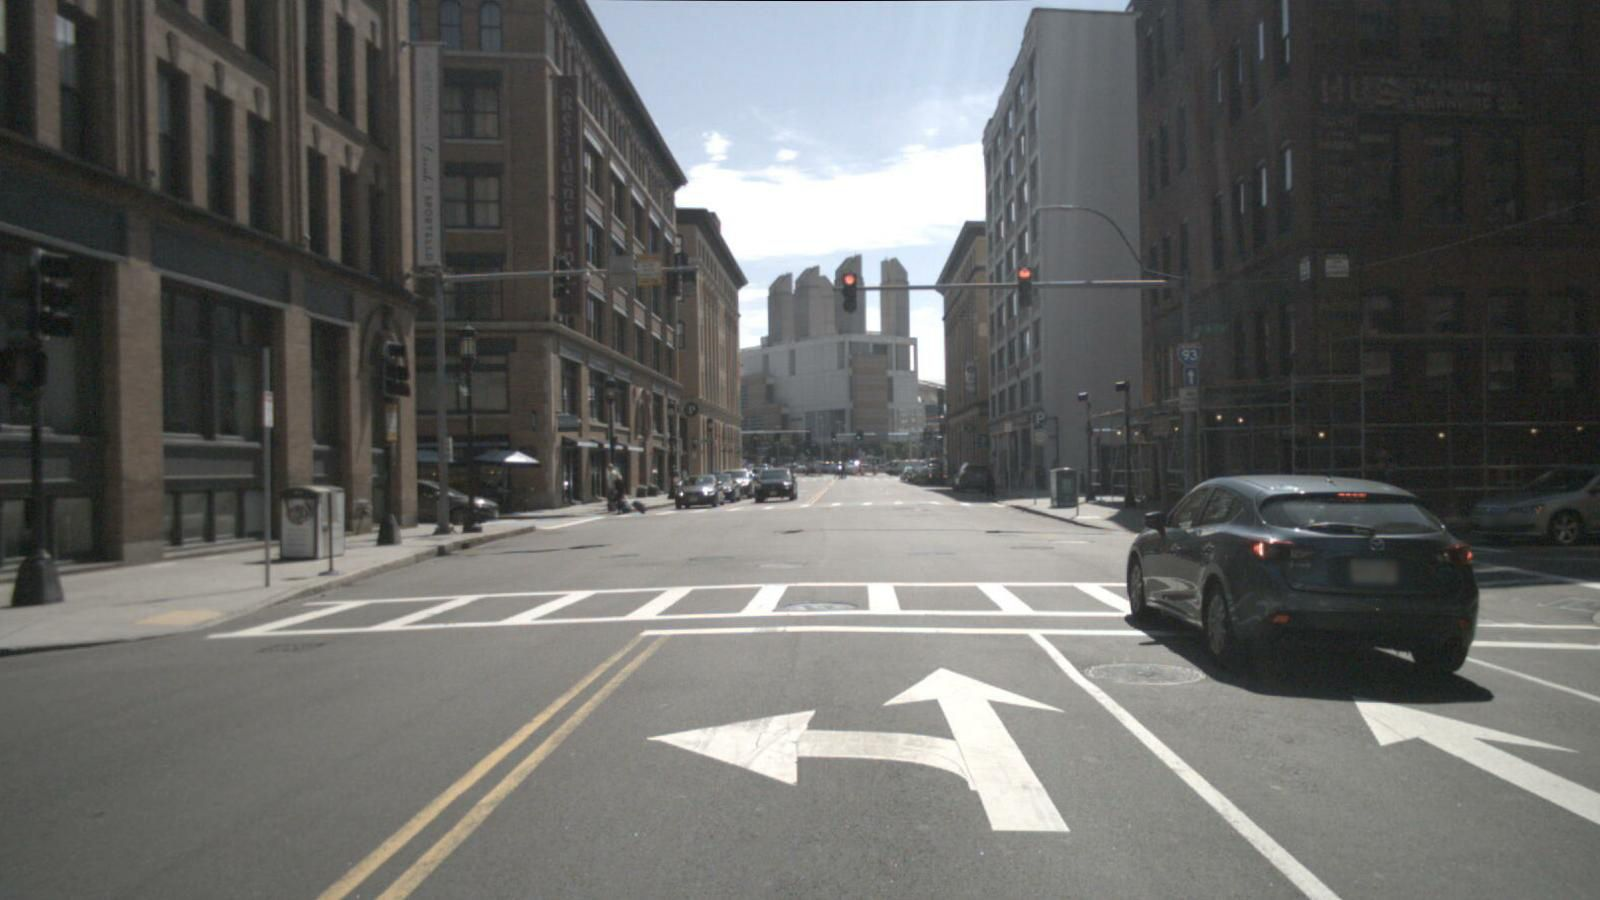
\includegraphics[width=0.8\textwidth]{Figs/depth_origin.jpg}
%     \caption{Original image in nuScenes dataset for depth generation}
%     \label{fig:depth_origin}
% \end{figure}
% \begin{figure}[tb!]
%     \centering
%     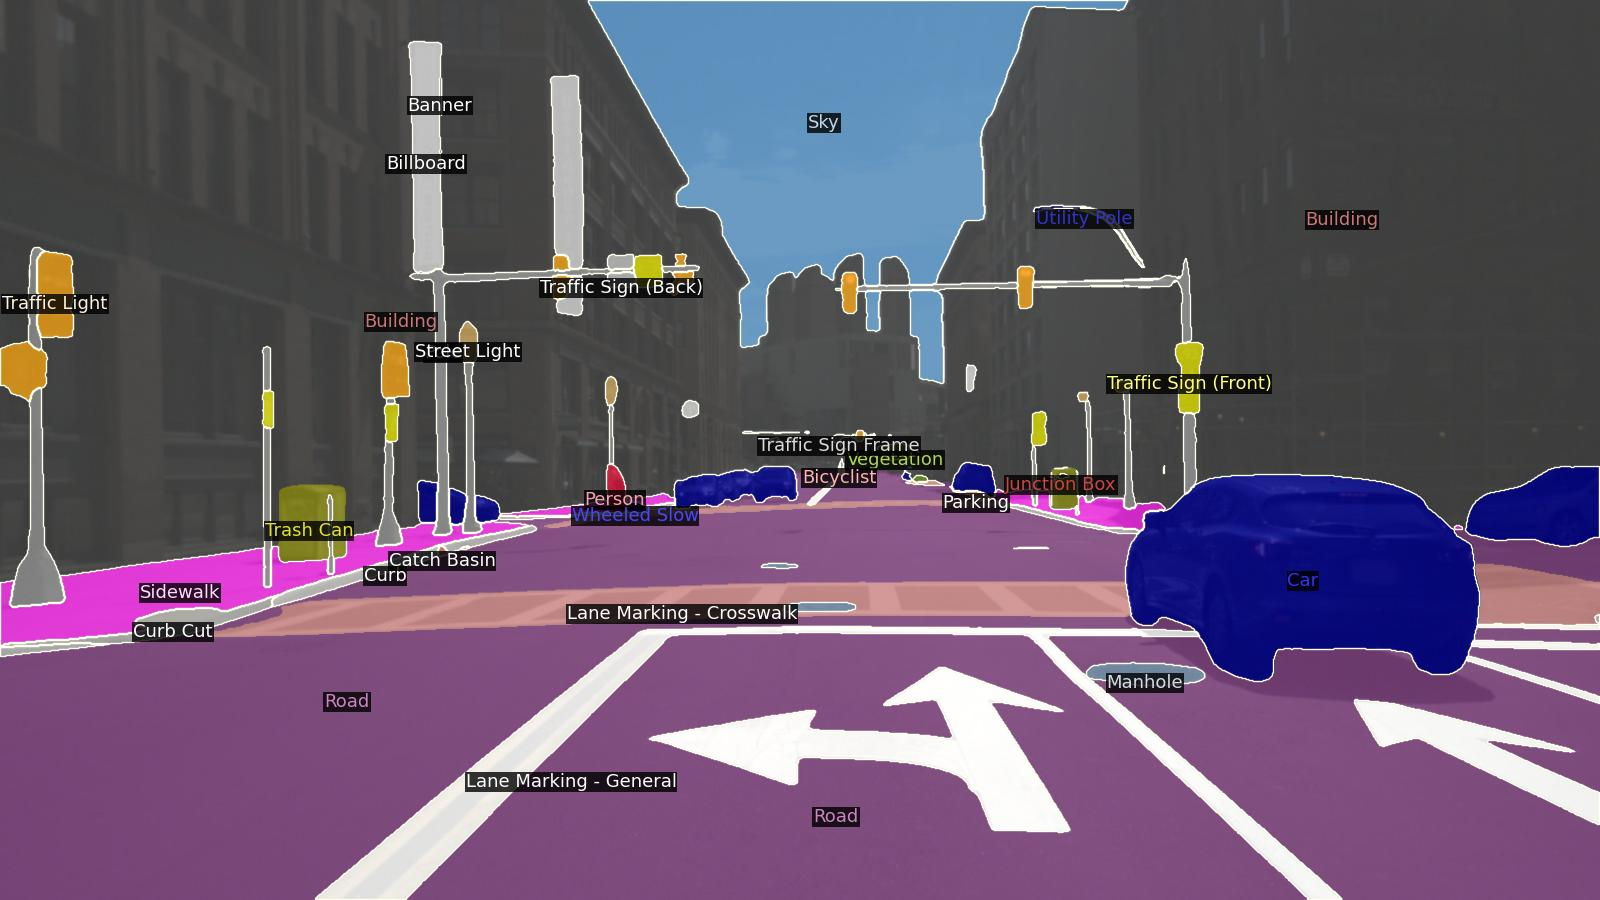
\includegraphics[width=0.8\textwidth]{Figs/depth_seg.jpg}
%     \caption{Segmentation result}
%     \label{fig:depth_seg}
% \end{figure}
% \begin{figure}[tb!]
%     \centering
%     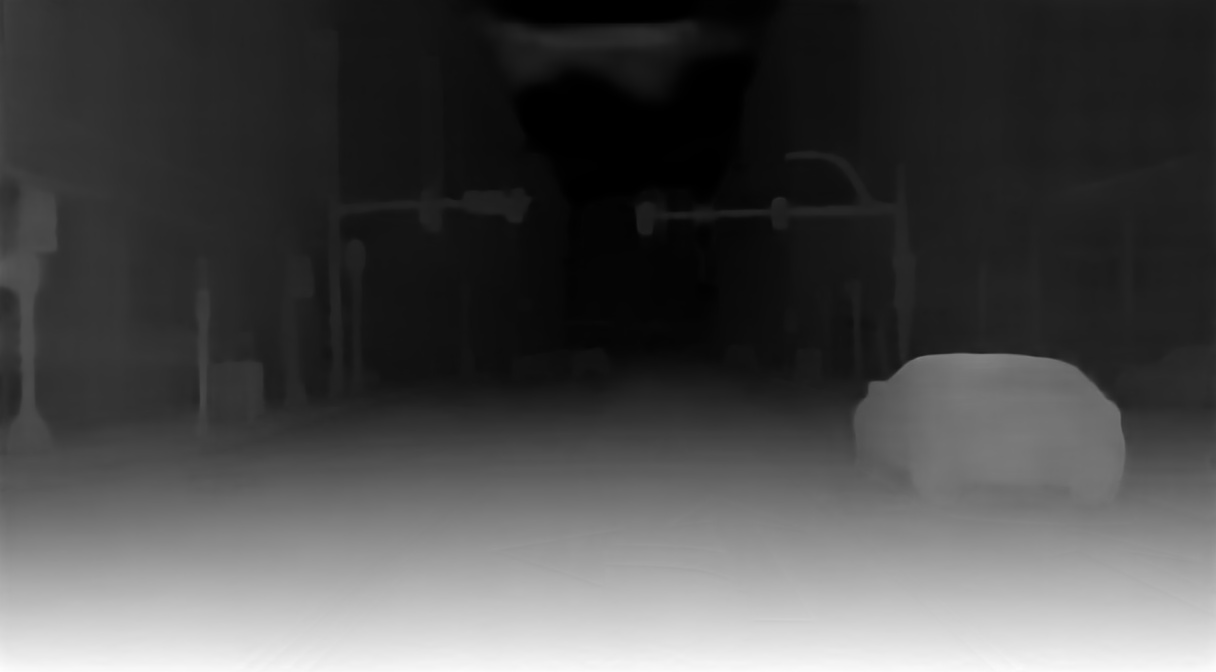
\includegraphics[width=0.8\textwidth]{Figs/depth_depth.jpg}
%     \caption{Predicted depth map}
%     \label{fig:depth_depn}
% \end{figure}


\begin{figure}[tb!]
    \centering
    \subfigure[]{
    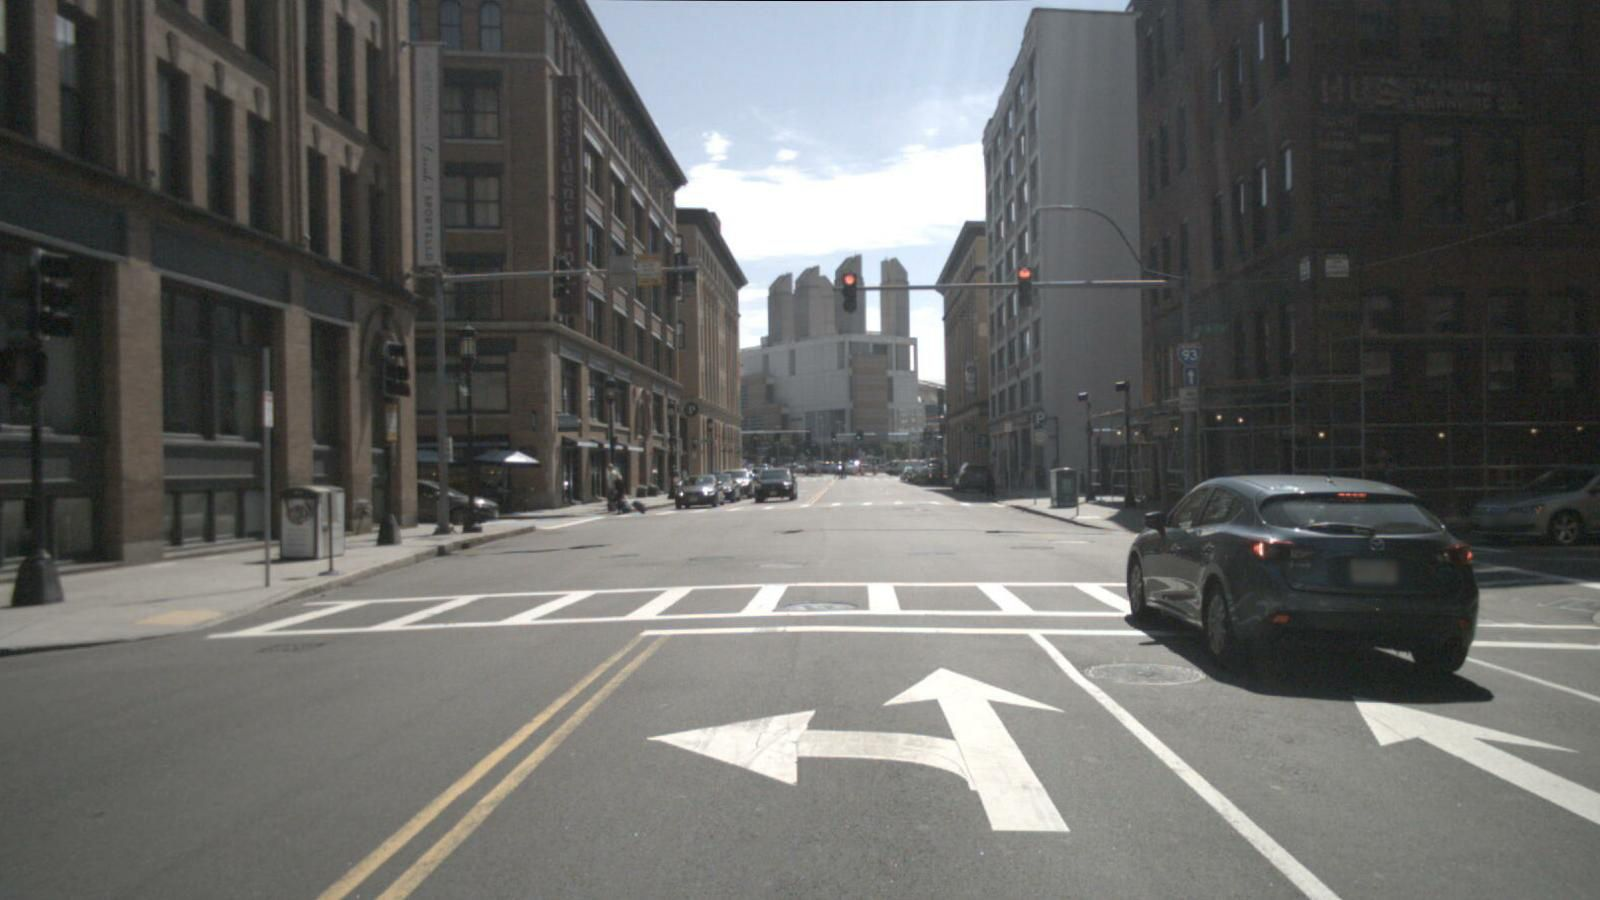
\includegraphics[width=0.75\textwidth]{Figs/depth_origin.jpg}
    }
    \quad
    \subfigure[]{
    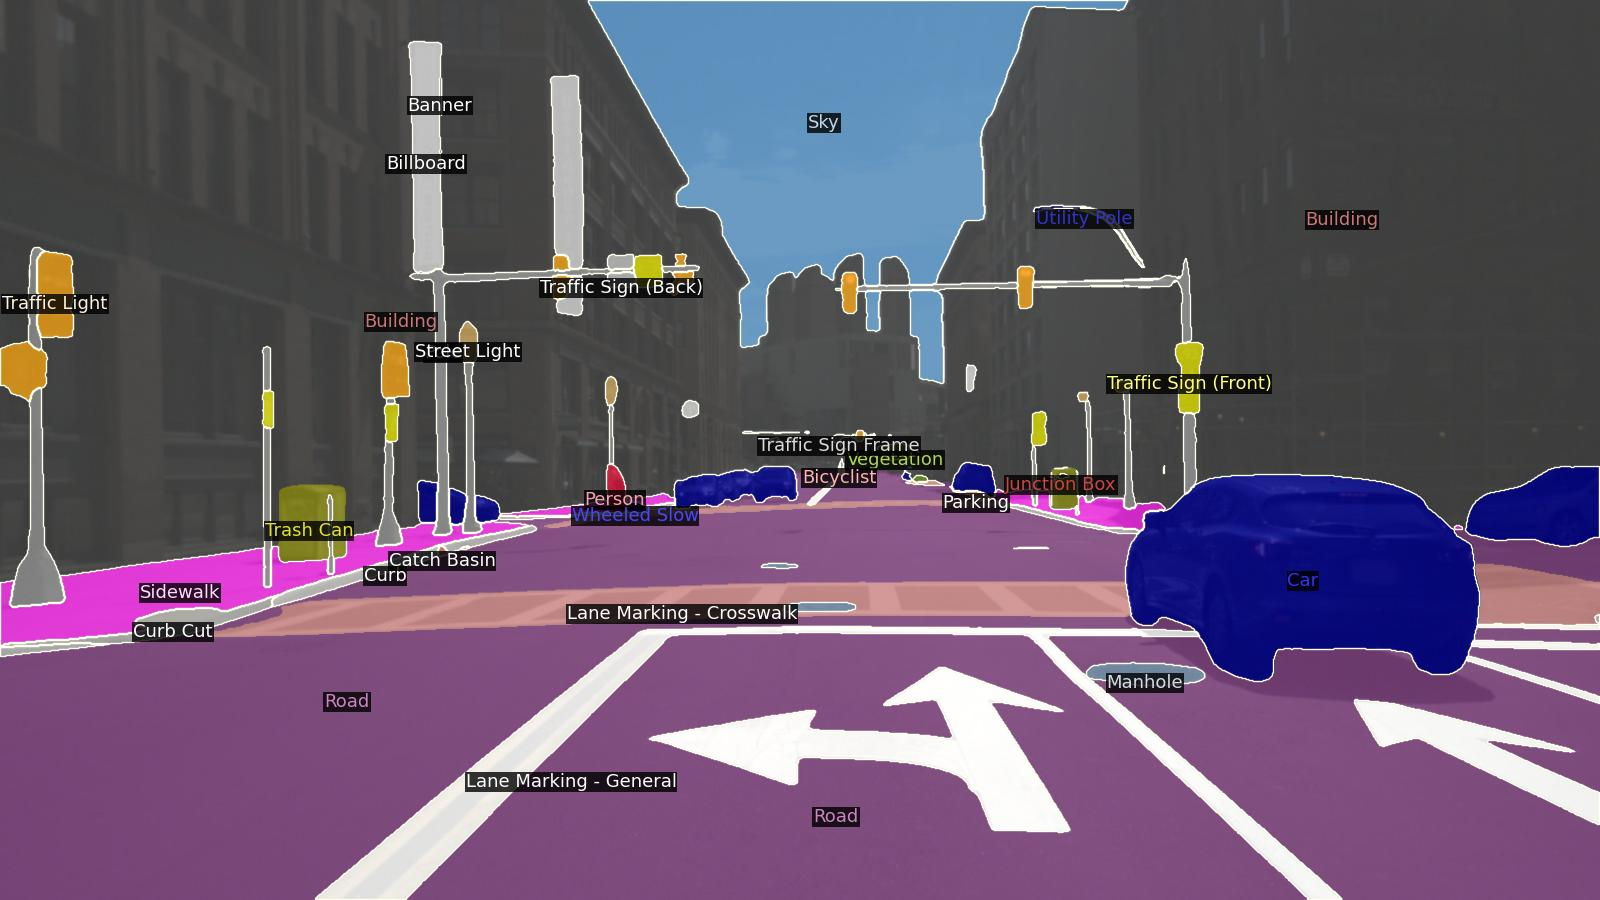
\includegraphics[width=0.75\textwidth]{Figs/depth_seg.jpg}
    }
    \quad
    \subfigure[]{
    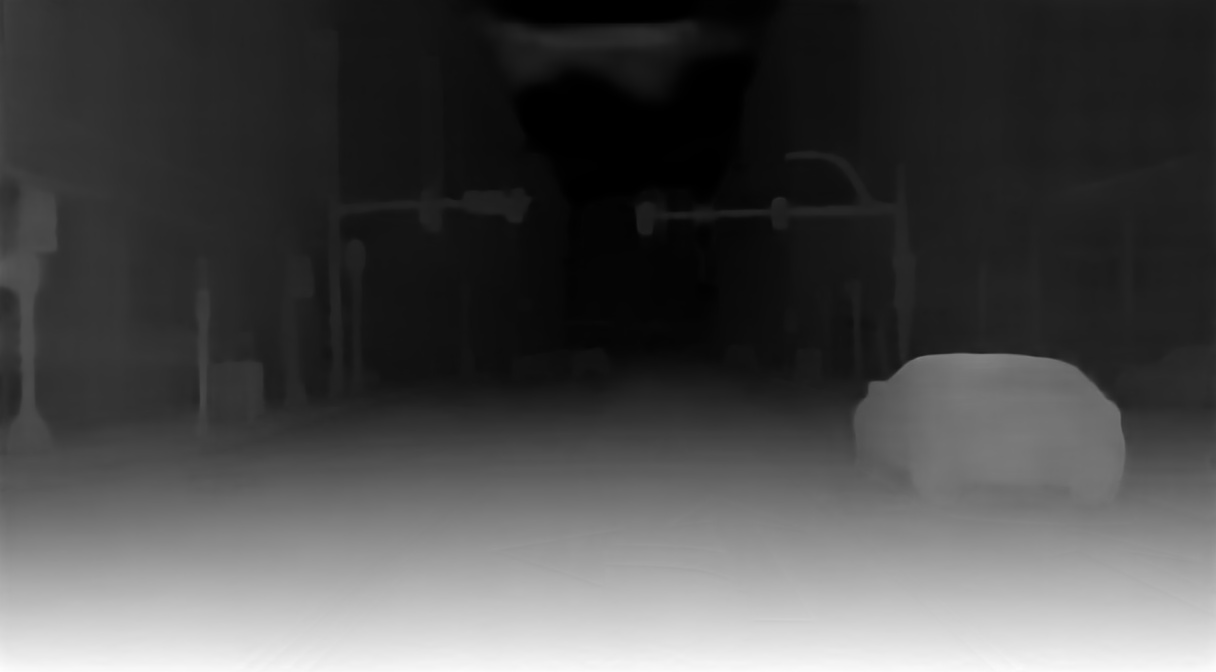
\includegraphics[width=0.75\textwidth]{Figs/depth_depth.jpg}
    }
    \caption{(a) 原始图像 (Original image); (b) 分割结果 (Segmentation result); (c) 预测深度图 (Predicted depth map)}
    \label{fig:depth_vis}
\end{figure}


% \begin{figure}[tb!]
%     \centering
%          \begin{subfigure}[b]{0.3\textwidth}
%              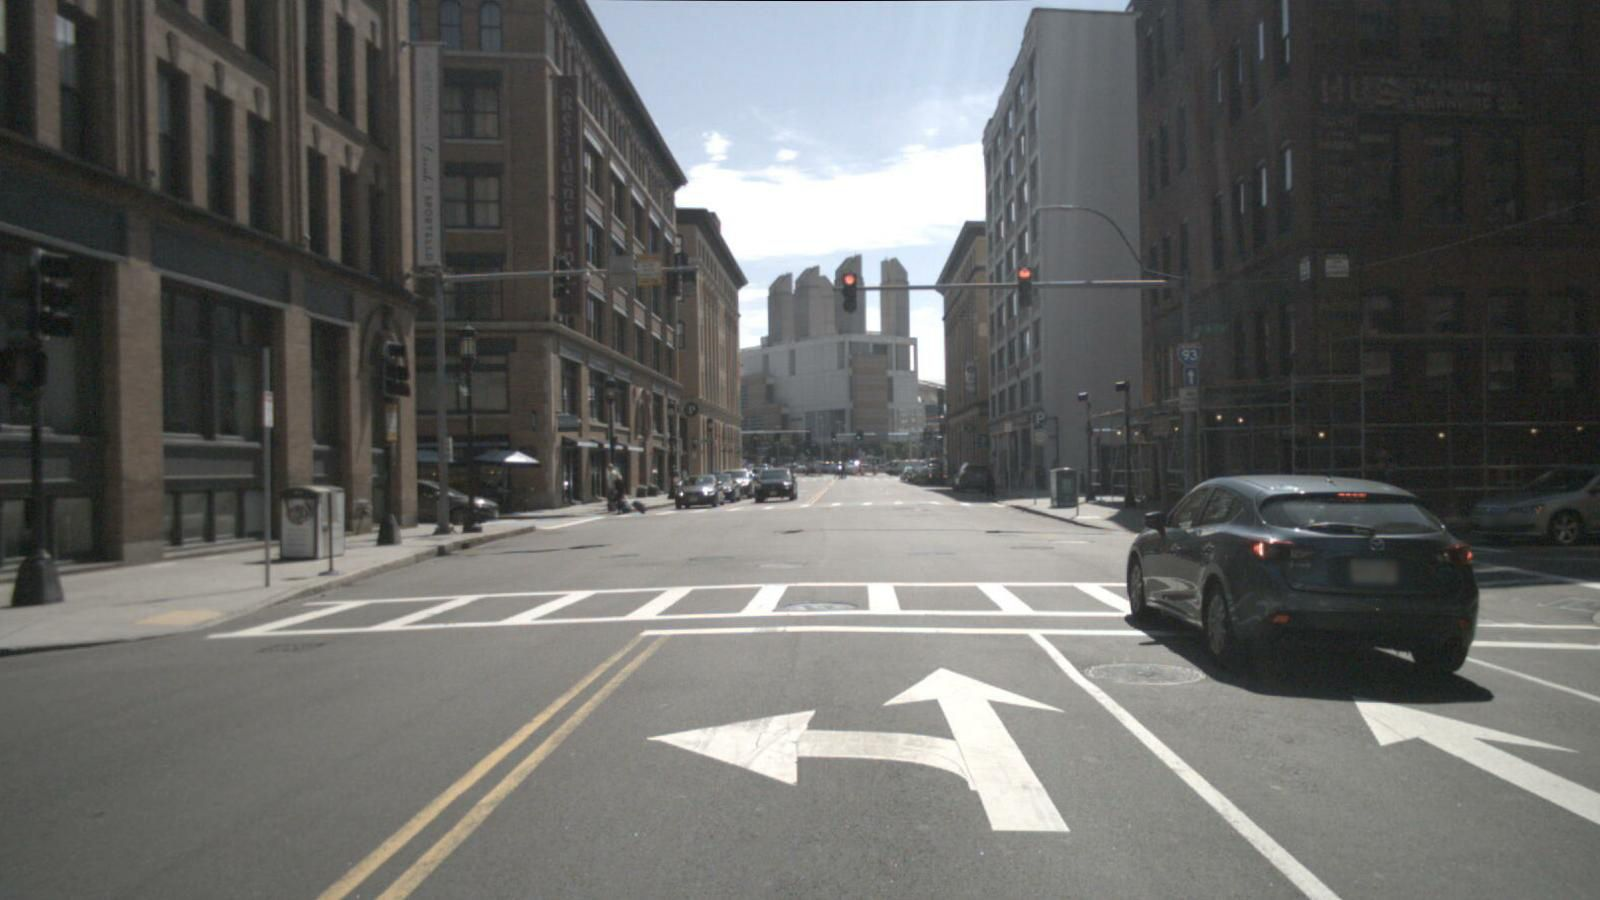
\includegraphics[width=0.3\textwidth]{Figs/depth_origin.jpg}
%              \caption{origin image}
%              \label{fig:depth_origin}
%          \end{subfigure}
         
%          \begin{subfigure}[b]{0.3\textwidth}
%              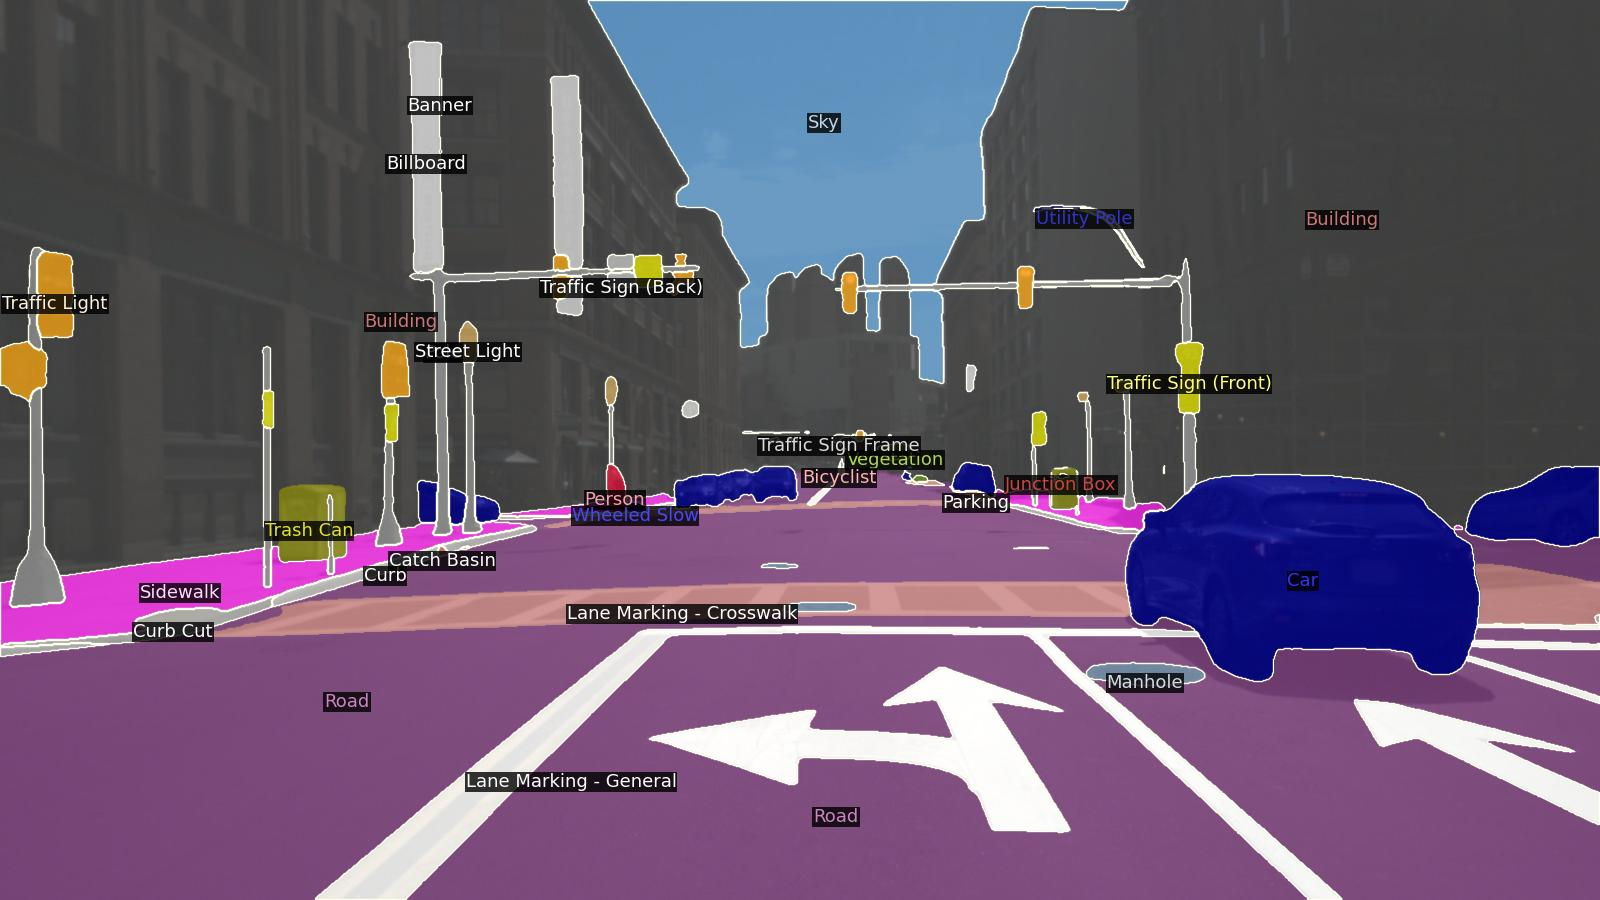
\includegraphics[width=0.3\textwidth]{Figs/depth_seg.jpg}
%              \caption{segmentation}
%              \label{fig:depth_seg}
%          \end{subfigure}
         
%          \begin{subfigure}[b]{0.3\textwidth}
%              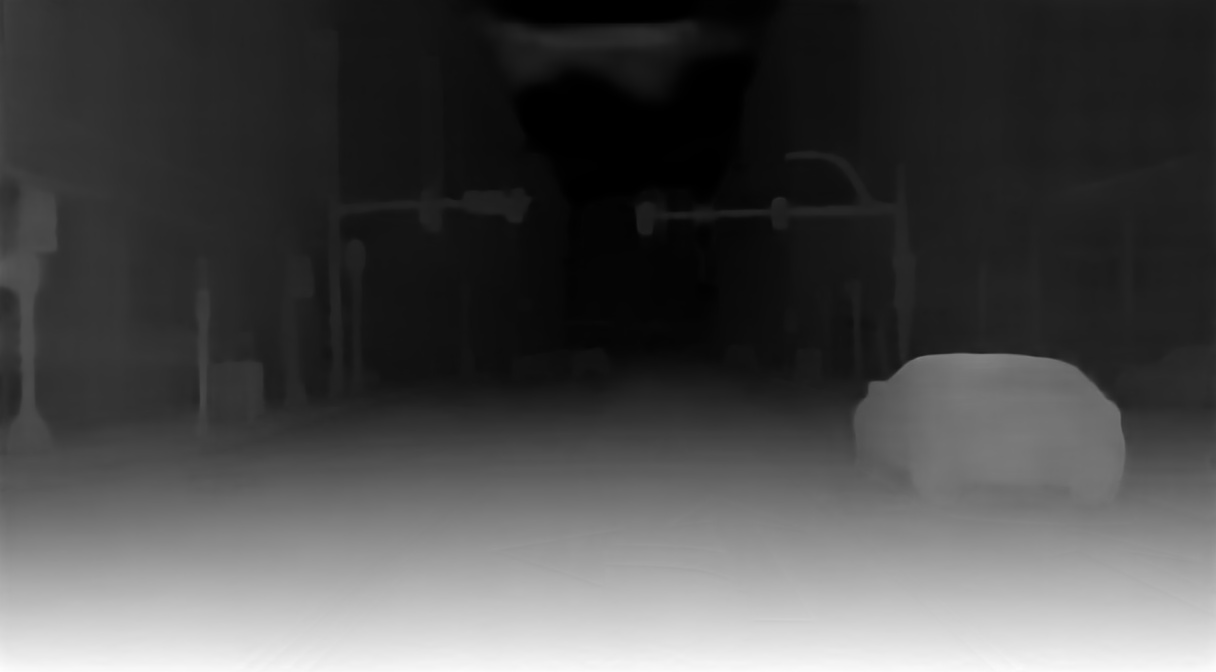
\includegraphics[width=0.3\textwidth]{Figs/depth_depth.jpg}
%              \caption{depth map}
%              \label{fig:depth_dep}
%          \end{subfigure}
%     \caption{visualization}
%     \label{fig:depth_vis}
% \end{figure}

\begin{table}[]
\centering
\caption{深度图评估 (Depth map evaluation). ARE：绝对相对误差 (absolute relative error)；SRE：平方相对误差 (square relative error)；RMSE：均方根误差 (root mean square error)；RMSE log：均方根对数误差 (root mean square logarithmic error)；$\delta$：精度 (accuracy, 阈值 1.25)}
\label{tab:depth_map_eval}
\scalebox{0.8}{
\begin{tabular}{p{0.2\textwidth}|>{\centering}p{0.13\textwidth}>{\centering}p{0.13\textwidth}>{\centering}p{0.13\textwidth}>{\centering}p{0.13\textwidth}>{\centering}p{0.13\textwidth}>{\centering}p{0.13\textwidth}>{\centering\arraybackslash}p{0.13\textwidth}}
\toprule
% \rowcolor[HTML]{C0C0C0} 
视角 (View) & ARE & SQE & RMSE   & RMSE log & $\delta$  & $\delta^2$  & $\delta^3$  \\ 
\midrule
FRONT       & 0.1522  & 3.5165 & 6.8756 & 0.2252   & 0.8720 & 0.9474 & 0.9701 \\
FRONT LEFT  & 0.2516  & 2.6591 & 5.7600 & 0.3035   & 0.7290 & 0.8755 & 0.9317 \\
FRONT RIGHT & 0.3030  & 5.9052 & 6.6903 & 0.3278   & 0.7067 & 0.8651 & 0.9231 \\
BACK        & 0.2297  & 5.5757 & 7.8486 & 0.3020   & 0.8011 & 0.9159 & 0.9535 \\
BACK LEFT   & 0.2752  & 3.6375 & 5.7691 & 0.3110   & 0.6982 & 0.8673 & 0.9279 \\
BACK RIGHT  & 0.3021  & 3.9396 & 6.2027 & 0.3413   & 0.6605 & 0.8503 & 0.9279 \\ \bottomrule
\end{tabular}}
\end{table}




\section{实验 (Experiments)}
\subsection{协议 (Protocols)}
\indent\textbf{数据集 (Dataset).}
在开环 (open-loop) 和闭环 (closed-loop) 环境下评估 ST-P3。%
%
采用 nuScenes 数据集~\cite{caesar2020nuscenes} 进行开环实验，CARLA 仿真器~\cite{dosovitskiy2017carla} 用于闭环演示。

对于 nuScenes，默认取过去 $1.0s$ 上下文，预测未来 $2.0s$ 上下文，对应过去 3 帧和未来 4 帧。
%
每个批次输入模型包含 7 帧上下文，按官方划分方法将数据集分为训练集和验证集，分别包含 26124 和 5719 个样本。

%
对于 CARLA，进行闭环评估。注意仍需要先以开环方式训练模型。
%
数据收集参照~\cite{prakash2021multi}，使用 Town05 场景进行评估，其余场景用于训练。
%
%
值得指出，CARLA 的相机配置仅包含 4 个相机，因此无法覆盖自动驾驶车辆 (SDV) 周围 $360^{\circ}$ 视场。
%
将过去 $1.0s$ 上下文和当前 4 个相机图像输入模型，生成轨迹并交由仿真器执行，直至 SDV 到达目的地或超时。
% The temporal setting is same as in nuScenes, but the spatial setting is $(40m, 40m)$ around SDV with resolution $(0.20m, 0.20m)$.


\noindent\textbf{实现细节 (Implementation Details).}
采用 EfficientNet-B4~\cite{tan2019efficientnet} 作为主干网络 (backbone)，详细模型描述见补充材料。使用 Adam 优化器，恒定学习率 $2 \times 10^{-4}$。在 4 块 Tesla V100 GPU 上以混合精度训练 20 个 epoch。
%
在 nuScenes 数据集上，BEV 空间范围为 SDV 周围 $(100m, 100m)$，分辨率 $(0.50m,0.50m)$，参照~\cite{hu2021fiery} 设置以公平比较。而在 CARLA 上，范围为 SDV 周围 $(40m, 40m)$，分辨率 $(0.20m, 0.20m)$。两个数据集相邻两帧时间间隔均为 0.5$s$。


\subsection{nuScenes 开环实验结果 (Open-loop Experimental Results on nuScenes)}

本节展示 nuScenes 数据集~\cite{caesar2020nuscenes} 上更多定性结果。同时展示学习到代价体 (cost volume) 和多种语义要素合成图的可视化。
%
注意颜色越深表示代价越小，反之亦然。如图 \ref{fig:nu_plan}-\ref{fig:nu_turning} 所示，汽车占据的位置基本都有较高代价，而可行驶开阔区域代价较低。

\begin{figure}[tb!]
    \centering
    \subfigure{
    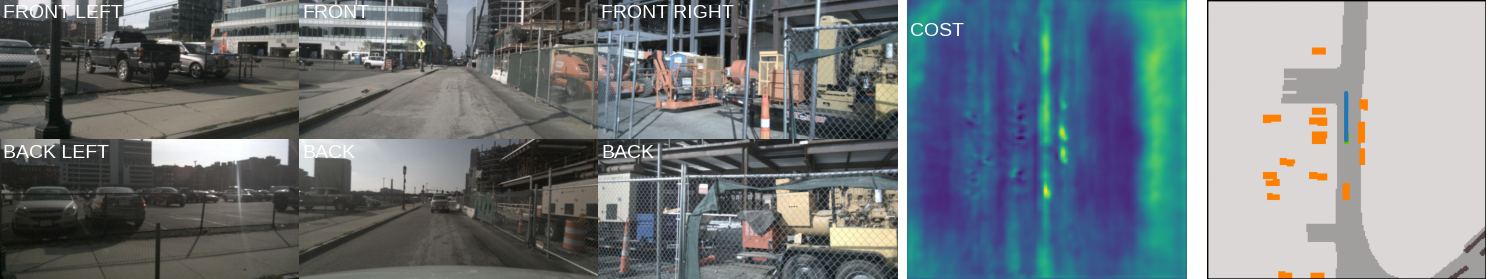
\includegraphics[width=0.98\textwidth]{Figs/nu_0319.png}
    }
    \quad
    \subfigure{
    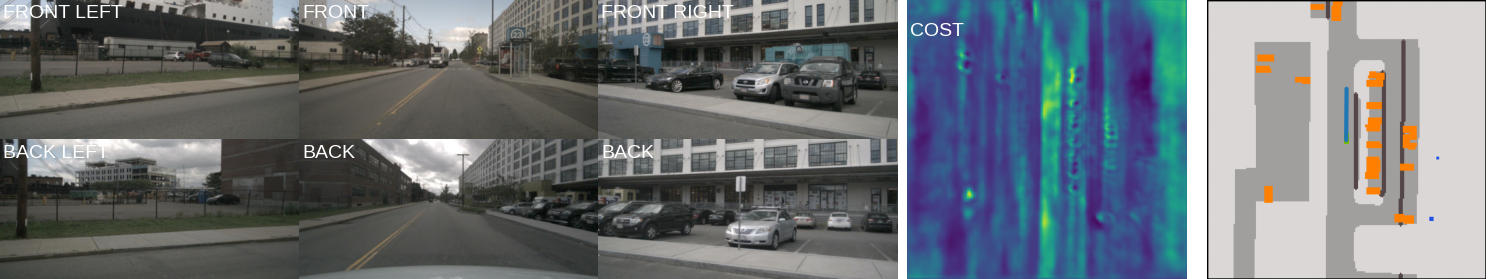
\includegraphics[width=0.98\textwidth]{Figs/nu_0169.png}
    }
    \quad
    \subfigure{
    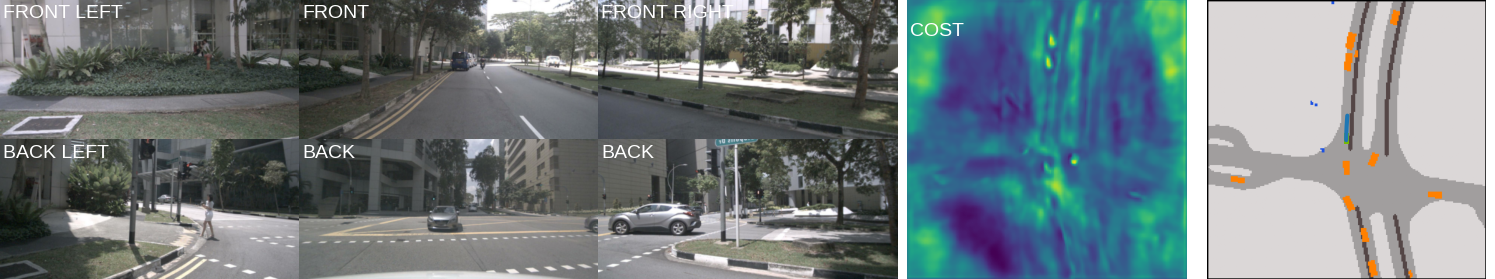
\includegraphics[width=0.98\textwidth]{Figs/nu_0295.png}
    }
    \caption{ST-P3 在直道上的定性结果 (Qualitative results of ST-P3 on the straight road)。右侧展示 BEV 中间表示和规划轨迹 (\textcolor{blue}{蓝色})，同时展示从预测模块学到子代价图。颜色越深表示代价越小}
    \label{fig:nu_plan}
\end{figure}

\begin{figure}[tb!]
    \centering
    \subfigure{
    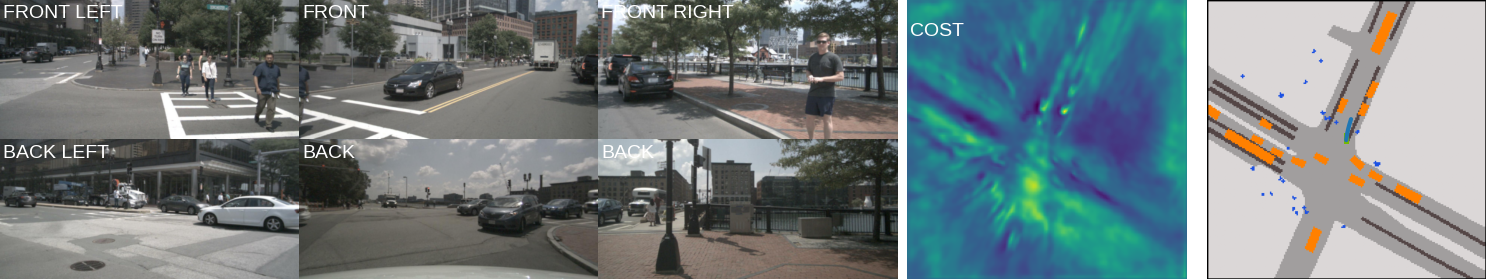
\includegraphics[width=0.98\textwidth]{Figs/nu_0021.png}
    }
    \quad
    \subfigure{
    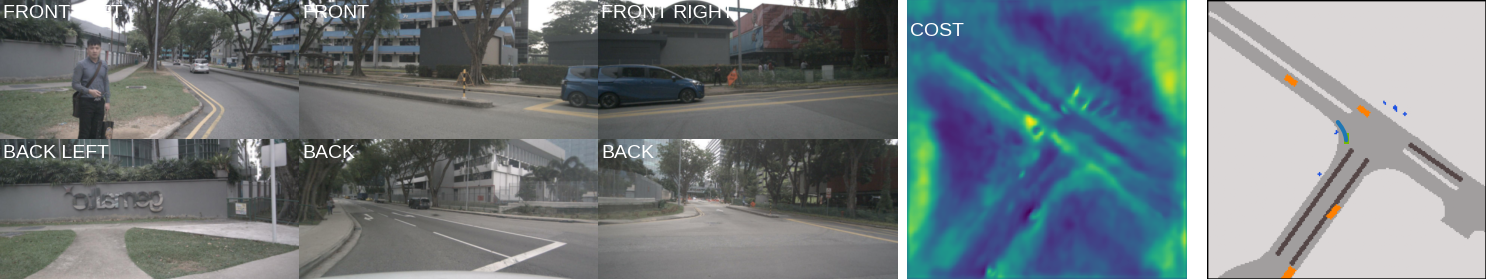
\includegraphics[width=0.98\textwidth]{Figs/nu_0044.png}
    }
    \quad
    \subfigure{
    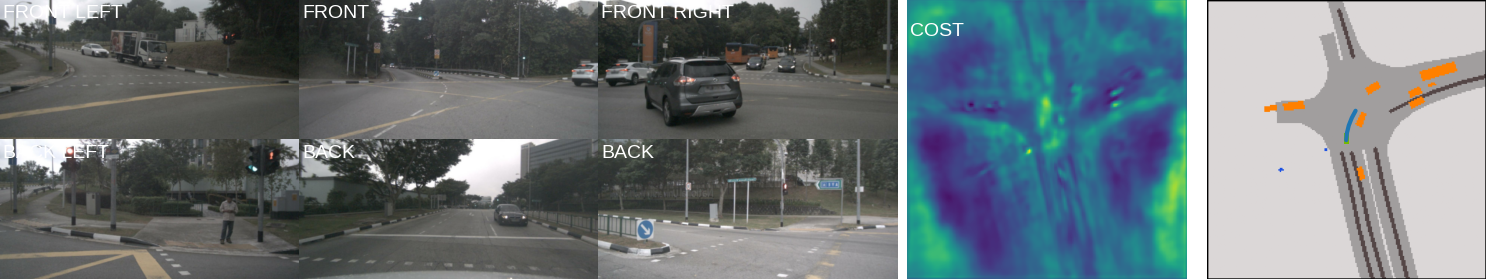
\includegraphics[width=0.98\textwidth]{Figs/nu_0376.png}
    }
    \caption{ST-P3 在交叉口转弯时的定性结果 (Qualitative results of ST-P3 when turning at intersections)}
    \label{fig:nu_turning}
\end{figure}

\subsection{CARLA 仿真器闭环规划结果 (Closed-loop Planning Results on CARLA Simulator)}
本节展示 CARLA 仿真器~\cite{dosovitskiy2017carla} 上定性结果，类似于开环结果。
%
如图 \ref{fig:error_recover} 所示，当车辆偏离车道中央时，地图检测精度显著下降。
%
这可能是由于大多数训练数据采集于正常行驶场景。
%
当地图精度较低时，使用采样器和代价图 (cost map) 的传统方法通常会偏离预期轨迹行为，但得益于优化 (refinement) 操作，车辆仍能正确行驶至预期轨迹。
%
更多不同场景可视化见图 \ref{fig:normal}-\ref{fig:turning}。

\begin{figure}[tb!]
    \centering
    \subfigure{
    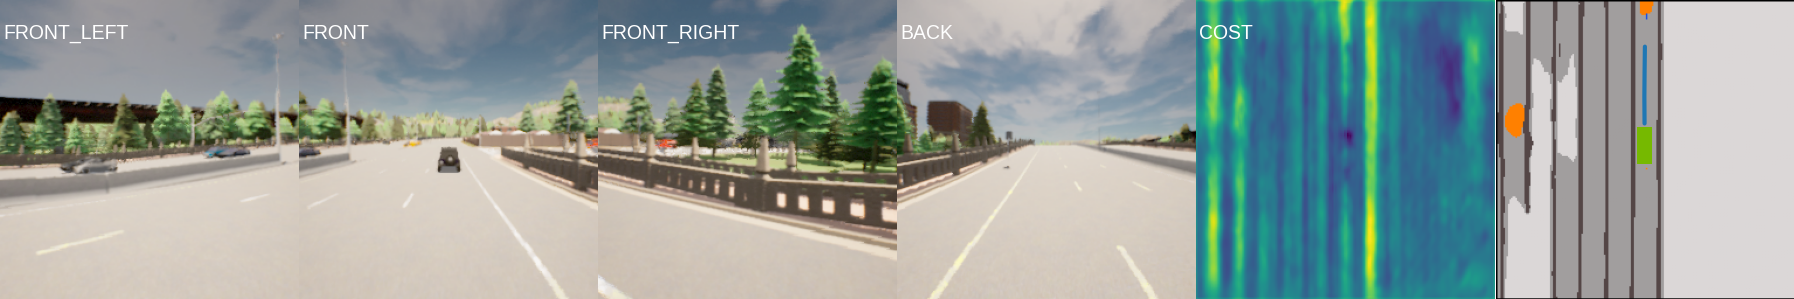
\includegraphics[width=0.98\textwidth]{Figs/0008.png}
    }
    \quad
    \subfigure{
    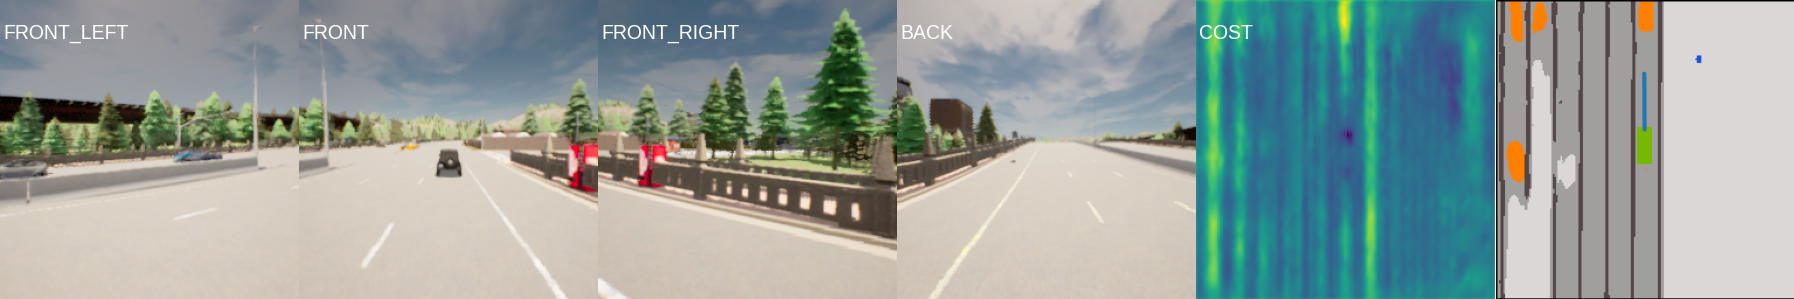
\includegraphics[width=0.98\textwidth]{Figs/0009.png}
    }
    \caption{ST-P3 在直道上的闭环规划定性结果 (Qualitative results of ST-P3 in closed-loop planning on the straight road)}
    \label{fig:normal}
\end{figure}

\begin{figure}[tb!]
    \centering
    \subfigure{
    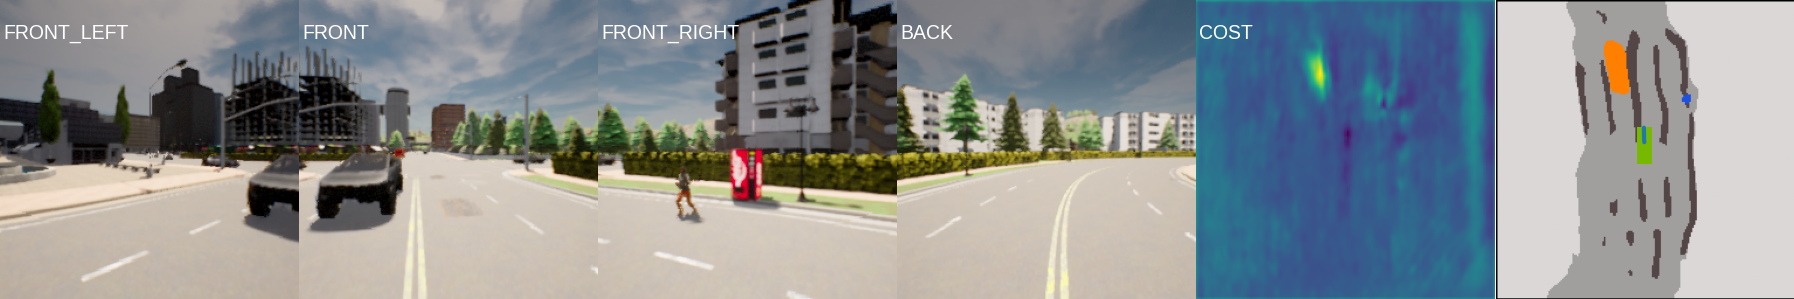
\includegraphics[width=0.98\textwidth]{Figs/0026.png}
    }
    \quad
    \subfigure{
    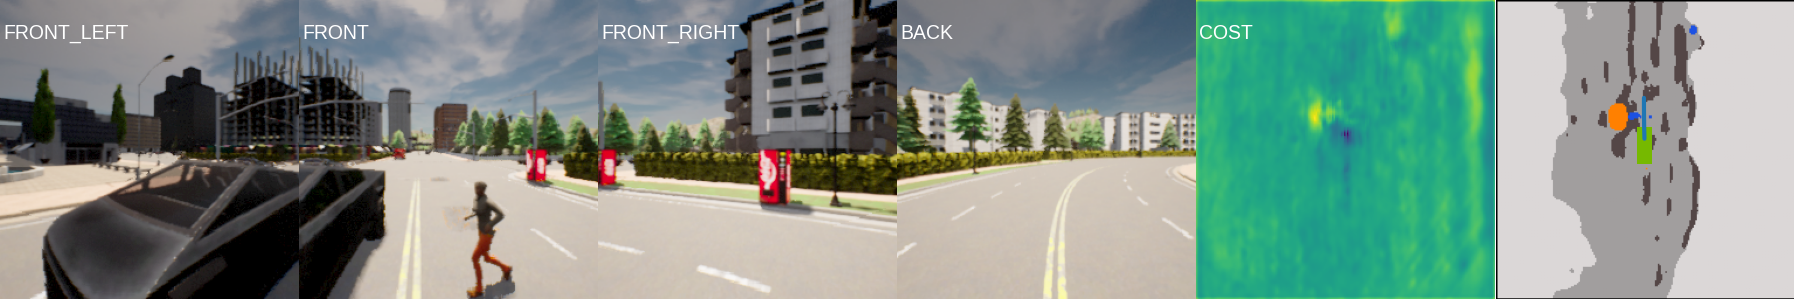
\includegraphics[width=0.98\textwidth]{Figs/0028.png}
    }
    \quad
    \subfigure{
    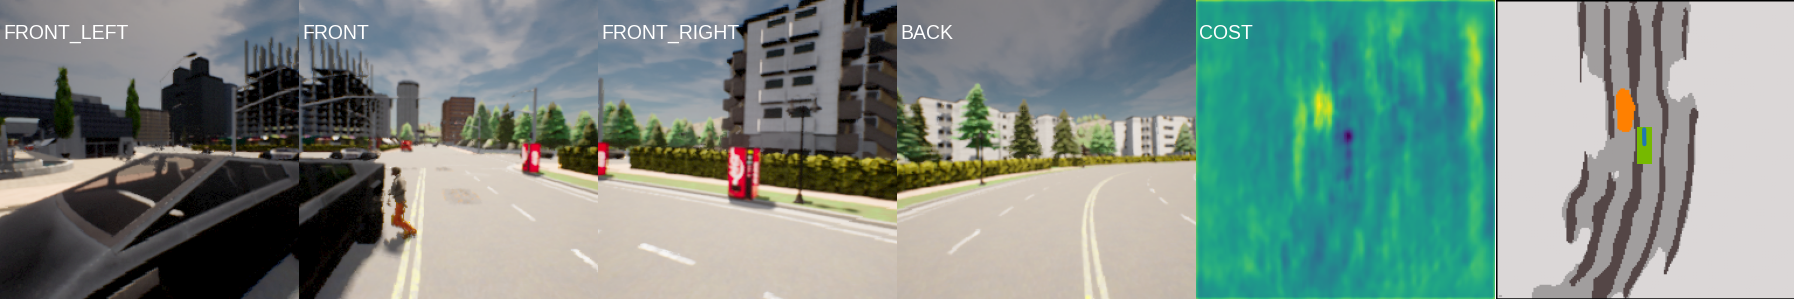
\includegraphics[width=0.98\textwidth]{Figs/0029.png}
    }
    \caption{检测到行人时 ST-P3 预测减速轨迹 (ST-P3 predicts a slowing down trajectory when detecting a pedestrian)}
    \label{fig:slow_down}
\end{figure}

\begin{figure}[tb!]
    \centering
    \subfigure{
    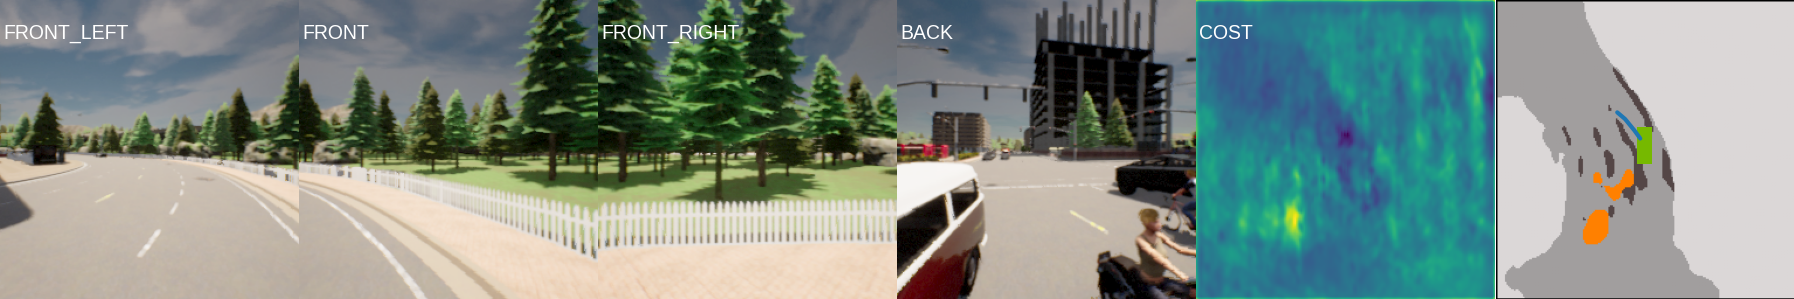
\includegraphics[width=0.98\textwidth]{Figs/0227.png}
    }
    \quad
    \subfigure{
    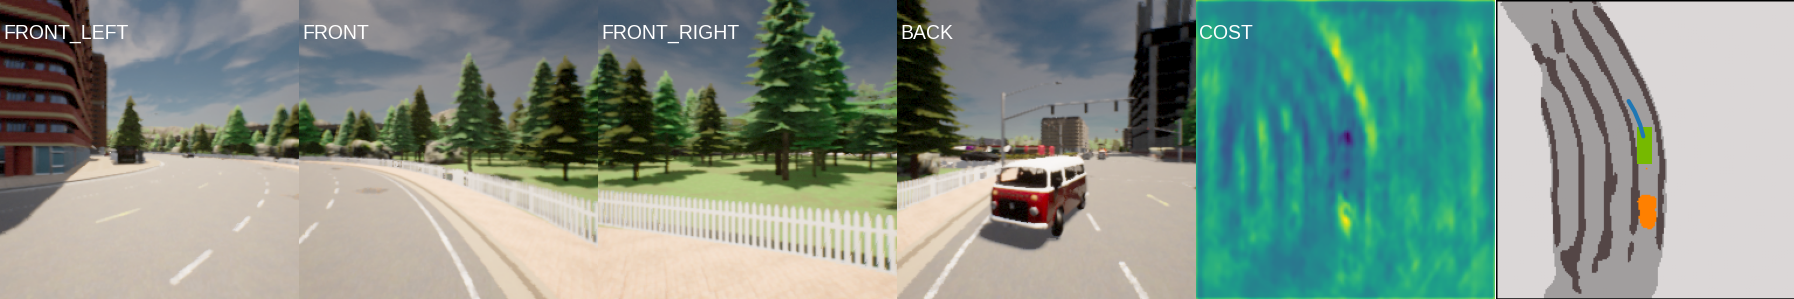
\includegraphics[width=0.98\textwidth]{Figs/0230.png}
    }
    \caption{沿预定轨迹（中心线）行驶时 ST-P3 的 BEV 表示恢复正常 (BEV representations of ST-P3 become normal when driving on a predetermined trajectory)}
    \label{fig:error_recover}
\end{figure}

\begin{figure}[tb!]
    \centering
    \subfigure{
    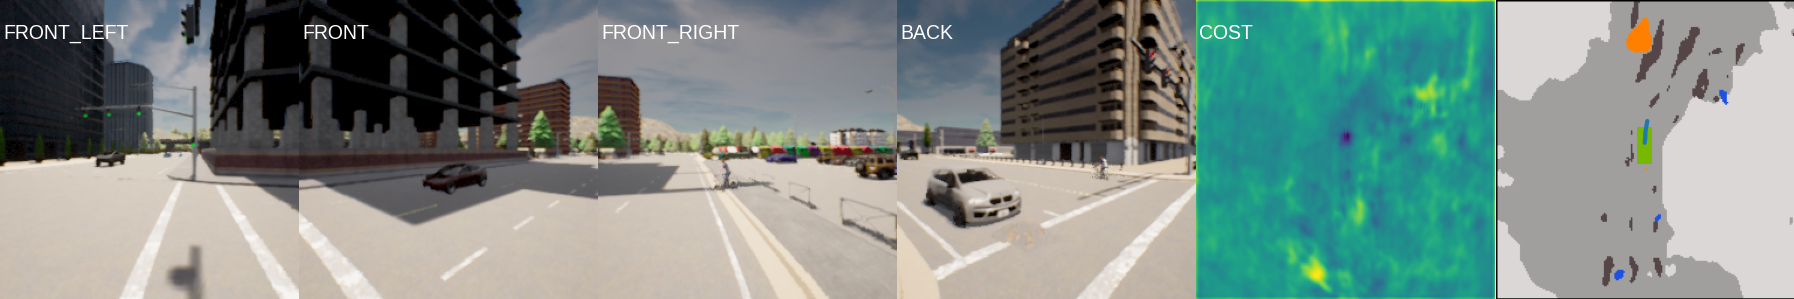
\includegraphics[width=0.98\textwidth]{Figs/0384.png}
    }
    \quad
    \subfigure{
    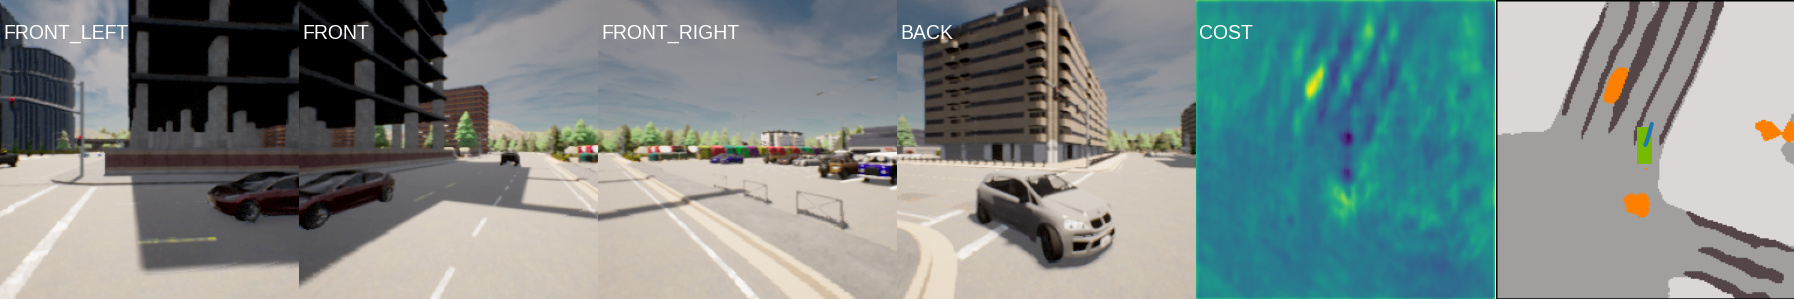
\includegraphics[width=0.98\textwidth]{Figs/0413.png}
    }
    \caption{ST-P3 在交叉口转弯时的闭环定性结果 (Qualitative results of ST-P3 in closed-loop when turning at intersections)}
    \label{fig:turning}
\end{figure}


% \input{sup}
% \section{Supplementary Materials}
% \subsection{Cost Function}
% \textbf{Safety Cost.} The SDV should not collide with other objects on the road and need to consider their future motion when planning its trajectory.
% %
% For this purpose, we use the predicted occupancy map to penalize the trajectories that intersect with the occupied regions.
% %
% % Thus, the prediction accuracy has a greater impact on the planning security, in our experiments we will illustrated the prediction accuracy at the same time.
% %
% Formally, for trajectories $\tau$ at each timestamp $t$, we will penalize $\tau$ if the SDV polygon $g$ intersects with the grids which are occupied by other objects (with a safety margin indicated by parameter $\lambda$), denoted by the $o_g(\tau, t, \lambda)$. The safety cost related to objects collision is given by: 
% \begin{equation}
%     f_o(\tau, o) = \sum_t \sum_g o_g(\tau, t, 0) + o_g(\tau, t, \lambda) v(\tau, t),
% \end{equation}
% where the first term penalizes the intersection grids whereas the second term penalizes the high-velocity motion with uncertainty occupancy.

% Moreover, SDV usually follows a leading vehicle and should keep a certain safe distance from it which mainly depends on the speed of the leading vehicle.
% %
% % In order to compute the headway cost, we should first find the leading vehicle and then compute the distance between it and SDV.
% %
% Since the HD map is unavailable and thus the leading vehicle along the center lane is unknown, instead we compute the occupancy grid in front of the SDV with a distance $L$ determined by the SDV velocity.
% %
% Hence if we are too close to the leading vehicle, the cost will be large that the trajectory will be evaluated as bad.
% %
% However it cannot take effect when it is in lane change manoeuvres since the leading vehicle is not directly in front of SDV.

% The above objectives focus on moving objects, meanwhile the vehicle should stay in the middle of the lane line as well.
% %
% We can ensure this traffic safety with the perceived lanes in the first stage, with a cost function that is set as the distance to lane lines.
% %Since we have no HD map information, we manually perceive the lane, but due to the limitation of accuracy, we cannot fully trust the result of the perception. Therefore, in order to adapt to this situation, we only consider the lane lines whose perception results exceed a certain probability. We should stay in the center of the lane line, that is, we should keep a certain distance from the lane line, so our cost function is set so that the closer to the lane line, the greater the cost value.

% \textbf{Cost Volume.} Due to the complexity of road information, we cannot manually enumerate all possible cases or planning cost, so we introduce a learned Cost volume generated by the aforementioned head as described in Sec.~\ref{sec: method-prediction}.
% %
% In order to balance the cost scale, we clip the cost volume value so that it does not take a dominant role in evaluating trajectories.

% \textbf{Comfort and Progress.} In terms of generating a smooth and comfortable trajectory, we penalize the trajectories with lateral acceleration, jerk and curvature.
% %
% What's more, we wish the trajectory is efficient to take the SDV to the target point, hence the trajectory progressing forward would be awarded.

\end{document}
